\documentclass[11pt]{article}
\usepackage[utf8]{inputenc}
\usepackage{amsmath, amssymb}
\usepackage{graphicx}
\usepackage{enumerate}
\usepackage{xcolor}
\usepackage{natbib}

\usepackage{caption}
\usepackage{subcaption}
\usepackage{float}
\usepackage[percent]{overpic}

\bibliographystyle{agsm.bst}

\usepackage{url} % not crucial - just used below for the URL 

%\pdfminorversion=4
% NOTE: To produce blinded version, replace "0" with "1" below.
\newcommand{\blind}{1}

% DON'T change margins - should be 1 inch all around.
\addtolength{\oddsidemargin}{-.5in}%
\addtolength{\evensidemargin}{-.5in}%
\addtolength{\textwidth}{1in}%
\addtolength{\textheight}{-.3in}%
\addtolength{\topmargin}{-.8in}%


% ----- used after frontpage stuff to change spacing ------
\def\spacingset#1{\renewcommand{\baselinestretch}%
{#1}\small\normalsize} \spacingset{1}
% --------------------------------------------------------

\newcommand{\mau}[1]{{\color{blue}{[Mauricio: #1]}}}
% \DeclareMathOperator*{\minimize}{minimize}
\begin{document}

% ------------ FRONTPAGE STUFF ------------------

\if1\blind
{
  \title{\bf Large-Scale Spatiotemporal Density Smoothing with the Graph-fused Elastic Net: Application to Ride-sourcing Driver Productivity Analysis}
  \author{\textbf{Mauricio Tec}\\
    Department of Statistics ad Data Sciences\\ University of Texas at Austin \vspace{.1cm} \\ 
    \textbf{James G. Scott}\\
    Department of Statistics ad Data Sciences\\ University of Texas at Austin \vspace{.1cm} \\
    \textbf{Natalia Zuniga-Garcia} \\
    Department of Civil, Architectural and Environmental Engineering \\
    University of Texas at Austin}
  \maketitle
} \fi

\if0\blind
{
  \bigskip
  \bigskip
  \bigskip
  \begin{center}
    {\LARGE\bf Large-Scale Spatiotemporal Density Smoothing for Ride-sourcing Driver Productivity Analysis}
\end{center}
  \medskip
} \fi

\bigskip
\begin{abstract}
We study an application of spatiotemporal density edge smoothing in large networks with sparse observations based on a graph-fused elastic net (GFEN). We use data from more than 1 million ride-sourcing trips in Austin, TX, which are scattered throughout a large graph of 223,944 nodes, representing each hour of the week and each traffic analysis zone (TAZ). We estimate a density model of the predicted productivity of a driver as defined in \citep{zuniga-etal-2018} for each node of the graph. We extend the methodology based on Pólya-tree decomposition and the graph-fused lasso (GFL) proposed in \citep{tansey-etal-2017} which is inapplicable to our case of study due to the sparsity of the data, as well as need for different smoothing parameters on the spatial and time directions. Our algorithm is well-suited for multi-threading and distributed computing. We provide the Julia package \texttt{GraphFusedSmoothing}\footnote{\url{https://github.com/mauriciogtec/GraphFusedSmoothing.jl}} to accompany this article.
\end{abstract}

\noindent%
{\it Keywords:}  graph-fused lasso, trend filtering on graphs, multi-scale density estimation, ride-sharing, large network analysis, Julia package
\vfill

% -------------------------------
\newpage
\spacingset{1.5} % DON'T change the spacing!

\section{Introduction}
\label{sec:intro}

Natalia: I will work on this part for problem, justification and so on.. 

\section{Methodology}
\label{sec:meth}
Don't take any of these section titles seriously.  They're just for
illustration.

\section{Simulation study}
\subsection{Data generation}
\subsection{Results}

\section{Case study: Spatiotemporal Density Smoothing for Ride-sourcing Driver Productivity Analysis}
\label{sec:casestudy}


\subsection{Ride-sourcing data}

We use data that the Austin-based non-profit transportation network company \textit{RideAustin} made publicly available in early 2017 \citep{dataworld-2017}. The dataset consists rides recorded between June 2nd, 2016 and April 13th, 2017. Each trip corresponds to a row in the database and includes information about origin and destination coordinates, starting and ending time, driver number, cost and request time. During this period \textit{RideAustin} had no major competition, since rival companies such as Uber and Lyft were temporarily restricted from operating in Austin.

Since the demand during the first month was limited, we restricted our analysis on data from September 1st, 2016 to April 13th, 2017. We selected rides having origin and destination coordinates within the traffic analysis zones\footnote{The TAZs are the unit of geography most commonly used in conventional transportation planning models.} (TAZs) of Austin. We only include regular car category trips; we omitted trips by sport-utility vehicles (SUV), premium, and luxury categories because the fare rate is different in each case. Similarly, we only analyzed flat-rate trips, i.e. trips that do not include any surge price. Finally, as we shall explain in the next section, we only consider trips in which the driver made a subsequent trip in within less than one hour. This is necessary to construct a measurement of productivity. The total number of rides examined based on the previous restrictions is 1,030,565 rides, with approximately 3,000 average daily trips. 

\begin{figure}[htb]
    \begin{minipage}[t]{.5\linewidth}
        \centering
        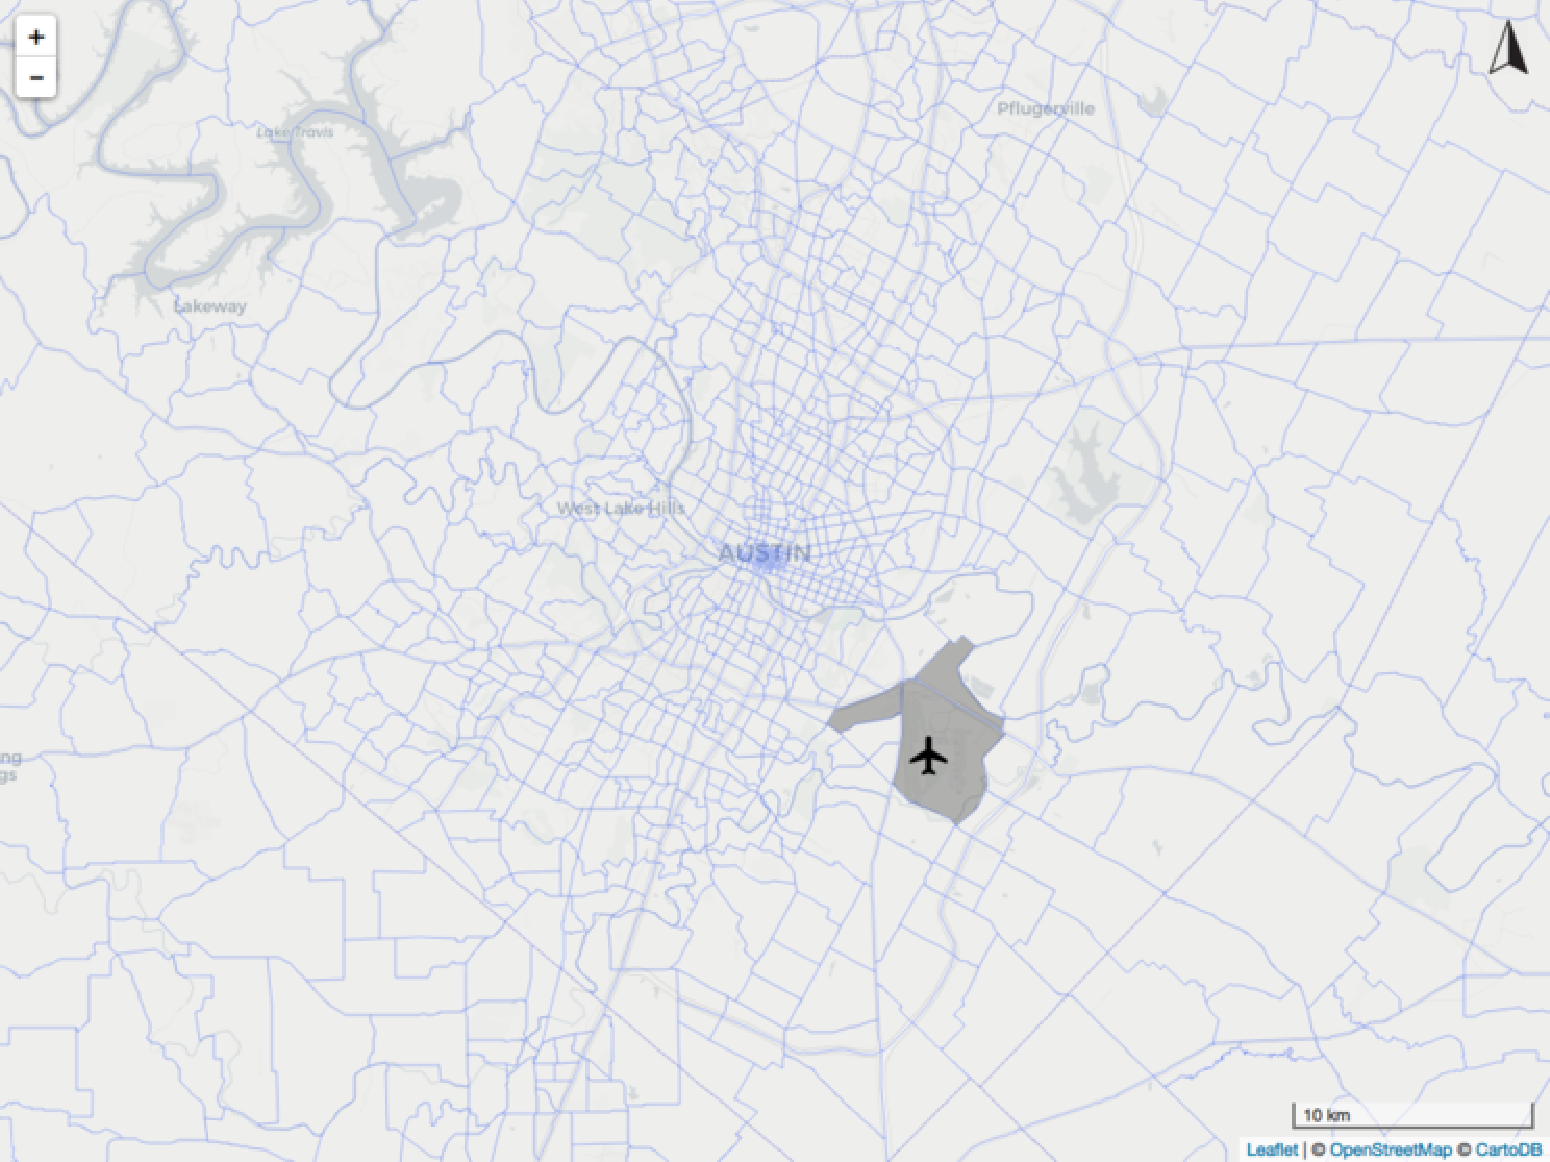
\includegraphics[width=0.99\linewidth]{img/tazs.pdf}
        \subcaption{TAZs in Austin (airport shaded)}
        \label{fig:areatypes:a}
    \end{minipage}%
    \begin{minipage}[t]{.5\linewidth}
        \centering
		\begin{overpic}[width=0.99\linewidth]{img/areatypes.pdf}
			\put(0,0){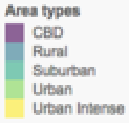
\includegraphics[scale=.25]{img/areatypes_legend.pdf}}
		\end{overpic}
		\subcaption{Area types}
		\label{fig:areatypes:b}
    \end{minipage}
    \caption{Description of TAZs. (a) shows the TAZs of Austin. Zones with less traffic tend to be larger. The airport is highlighted in gray. (b) shows the TAZs classified by area type. The central business district, which contain the downtown, is shown in purple.} \label{fig:areatypes}
\end{figure}



\subsection{Measuring productivity}

To measure driver productivity, we take a slight variation of the approach defined in \citep{zuniga-etal-2018}. This measurement is taken \textit{prospectively} from the driver's future rides. For each trip $i$, we denote:
\begin{itemize}\itemsep0em 
    \item $\mathtt{idle}_i$: the time in hours that the driver of trip $i$ will wait until beginning a subsequent trip; during this time the driver does not generate any revenue.
    \item $\mathtt{durnext}_i$: the time in hours that the \underline{same driver} of trip $i$ will take to complete the subsequent trip; during this time the driver is generating revenue determined by the tariff system.
    \item $\mathtt{farenext}_i$: the final fare of the subsequent trip; it is a function of a distance and a time tariff rate; \textit{c.f.} \citep{zuniga-etal-2018} for more details.
\end{itemize}
Our variable of interest is then defined as 
\begin{equation}
    \label{eq:productivity-def}
    \mathtt{productivity}_i := \frac{\mathtt{farenext}_i}{\mathtt{idle}_i + \mathtt{durnext}_i}
\end{equation}
Expression \eqref{eq:productivity-def} yields an interesting definition of productivity because it combines the time that the driver will stay unproductive with the quality of the subsequent trips. Moreover, its values are given naturally in dollars/hour. The idea is that when a trip ends, the driver starts searching for new riders. This prospective measurement gives the expected earnings given that a driver is at the specific location and time at which the last trip ended. If a trip ends in a location of low demand, the idle time will be large, but also subsequent trips could be longer. We remark that this definition deliberately ignores the fare trip that led to that position.

\begin{figure}[htb]
    \centering
    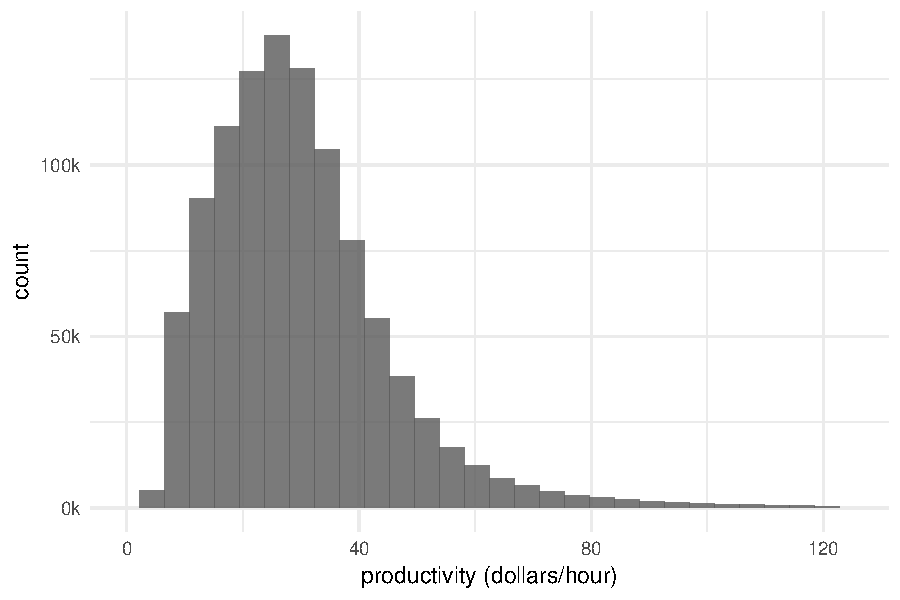
\includegraphics[width=0.65\linewidth]{img/prodhist_global.pdf}
    \caption{Histogram of productivity considering all trips}
    \label{fig:prodhist}
\end{figure}

We only considered trips in which the waiting time for a subsequent trip was less than one hour. This was necessary in order to exclude the cases where the driver took a meal break or stopped working for the day. Since during the time of data collection RideAustin did not have a major competing company, we do not have problems with long inter-trip times due to app switching. Figure \ref{fig:idledist} shows the distribution of the idle time in between trips after preprocessing and its distribution across TAZs.


\begin{figure}[htb]
    \centering
    \begin{minipage}[t]{.8\linewidth}
        \centering
        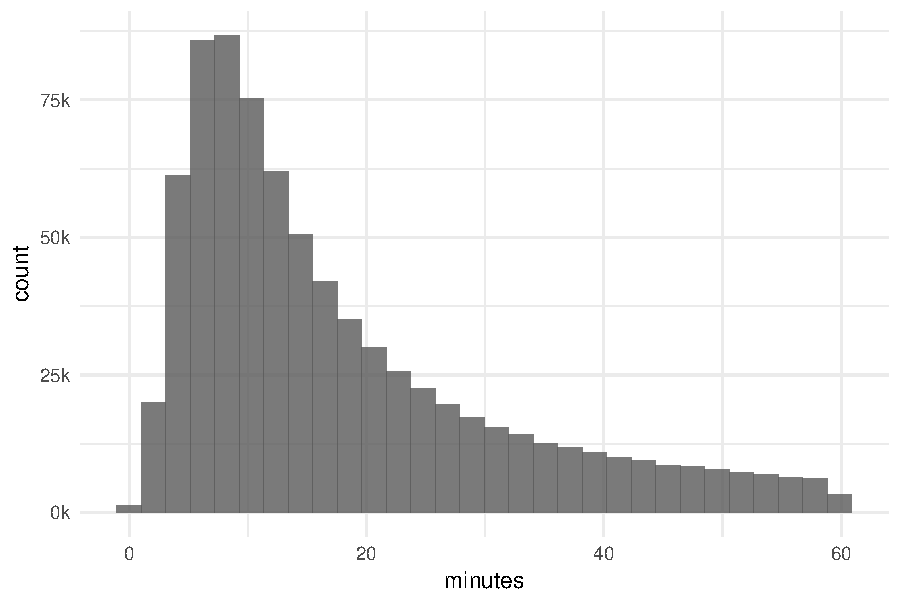
\includegraphics[width=0.8\linewidth]{img/idletime_hist.pdf}
        \subcaption{Distribution of idle time after trip end}
        \label{fig:idlehist}
    \end{minipage}\hfill
    \begin{minipage}[t]{.8\linewidth}
        \centering
        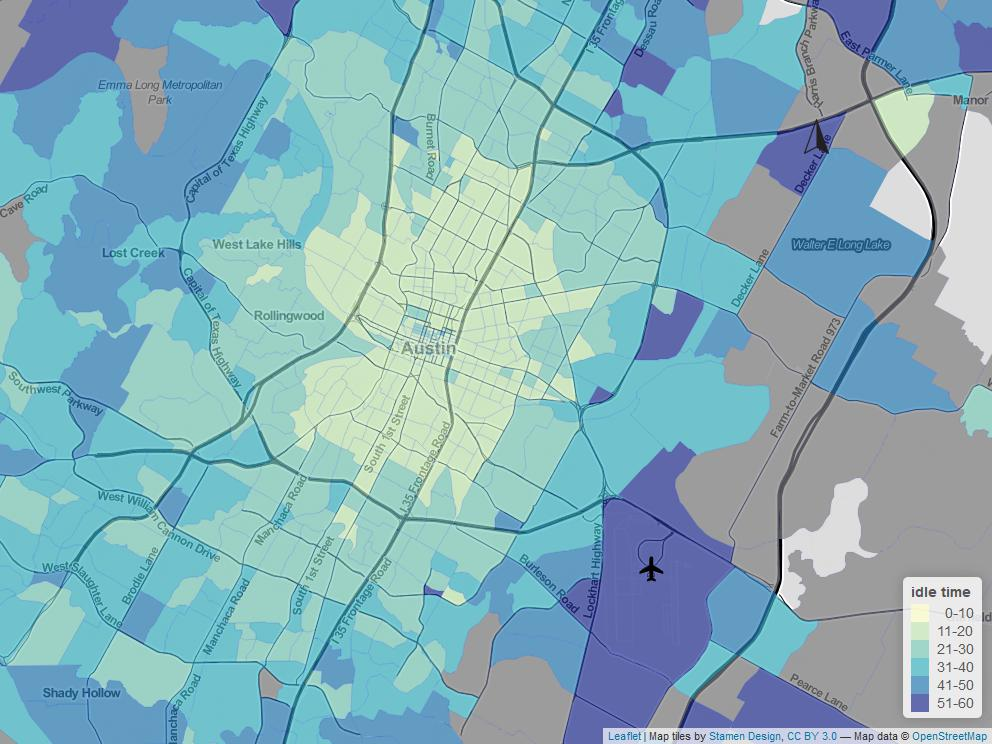
\includegraphics[width=0.8\linewidth]{img/idletime_spatial.jpeg}
        \subcaption{Median idle minutes in between trips by TAZ}
        \label{fig:idlemap}
    \end{minipage}%
    \caption{Histogram of productivity considering all trips}
    \label{fig:idledist}
\end{figure}


\subsection{Space and time discretization}

The TAZs of Austin are shown in Figure \ref{fig:areatypes}. The advantage of using them over a regular grid discretization is that their size vary accordingly to the traffic intensity, which is highly correlated to the number of trips present in the dataset. We thus have a high resolution near downtown and a low resolution in more rural areas. A total of $1333$ TAZs were considered, requiring that at least one trip originated or ended in that location. Time was discretized hourly, with a periodicity of one week. This results in $168=24\times7$ time periods.

Altogether, we considered $223944=168\times1333$ units of observation, which we used as the vertices of an undirected spatiotemporal graph. The node set of the graph is thus $V=
\left\{v_{st} \mid s=1,\hdots,1333, t=1,\hdots,168\right\}$.

Figure \ref{fig:prod_spacetime} shows the total counts of trips aggregating marginally for each time unit and for each space unit. When considered marginally, all space units and all time units have some data. However, once we split by both space and time, only 102600 of the 223944 nodes (45.8\%) have some data. This sparsity pattern motivates the use of our  elastic net method. 

We construct a set of edges $E$ as the union of a disjoint set of spatial and temporal edges $E=E_S\cup E_T$. The set $E_S$ of edges in the spatial direction was constructed geographically, drawing an edge $v_{s,t} \longleftrightarrow v_{r,t}$ for all pairs  $
\{s, r\}$ of adjacent TAZs. We excluded a few TAZs that were not in the largest connected component of the graph. Edges in the temporal direction $E_T$ were built as follows: given a node $v_{s,t}$ at location $s$ and time $t$, we drew edges $v_{s,t-1} \longleftrightarrow v_{s,t}$ and $v_{s,t} \longleftrightarrow v_{s,t+1}$ connecting a vertex with its subsequent and precedent observation. An extra edge $v_{s,168} \longleftrightarrow v_{s,1}$ was added for each site $s$, to account for the weekly periodicity. 



\begin{figure}[htb]
    \centering
    \begin{subfigure}[a]{.95\linewidth}
        \centering
        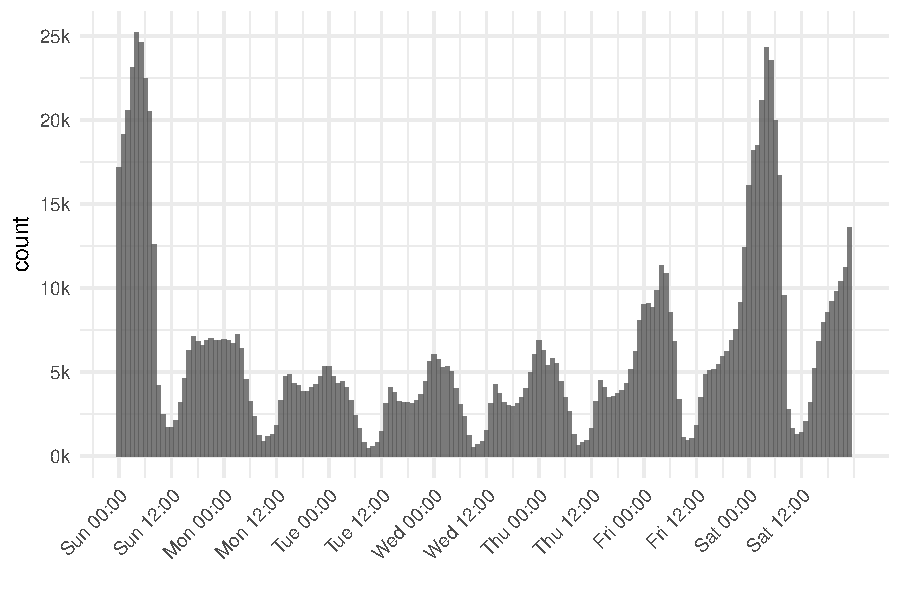
\includegraphics[width=0.7\linewidth]{img/prodhist_timely.pdf}
        \caption{Counts aggregated by time units}
        \label{fig:prod:timely}
    \end{subfigure}%\\
    \hfill
    \begin{subfigure}[b]{.95\linewidth}
        \centering
        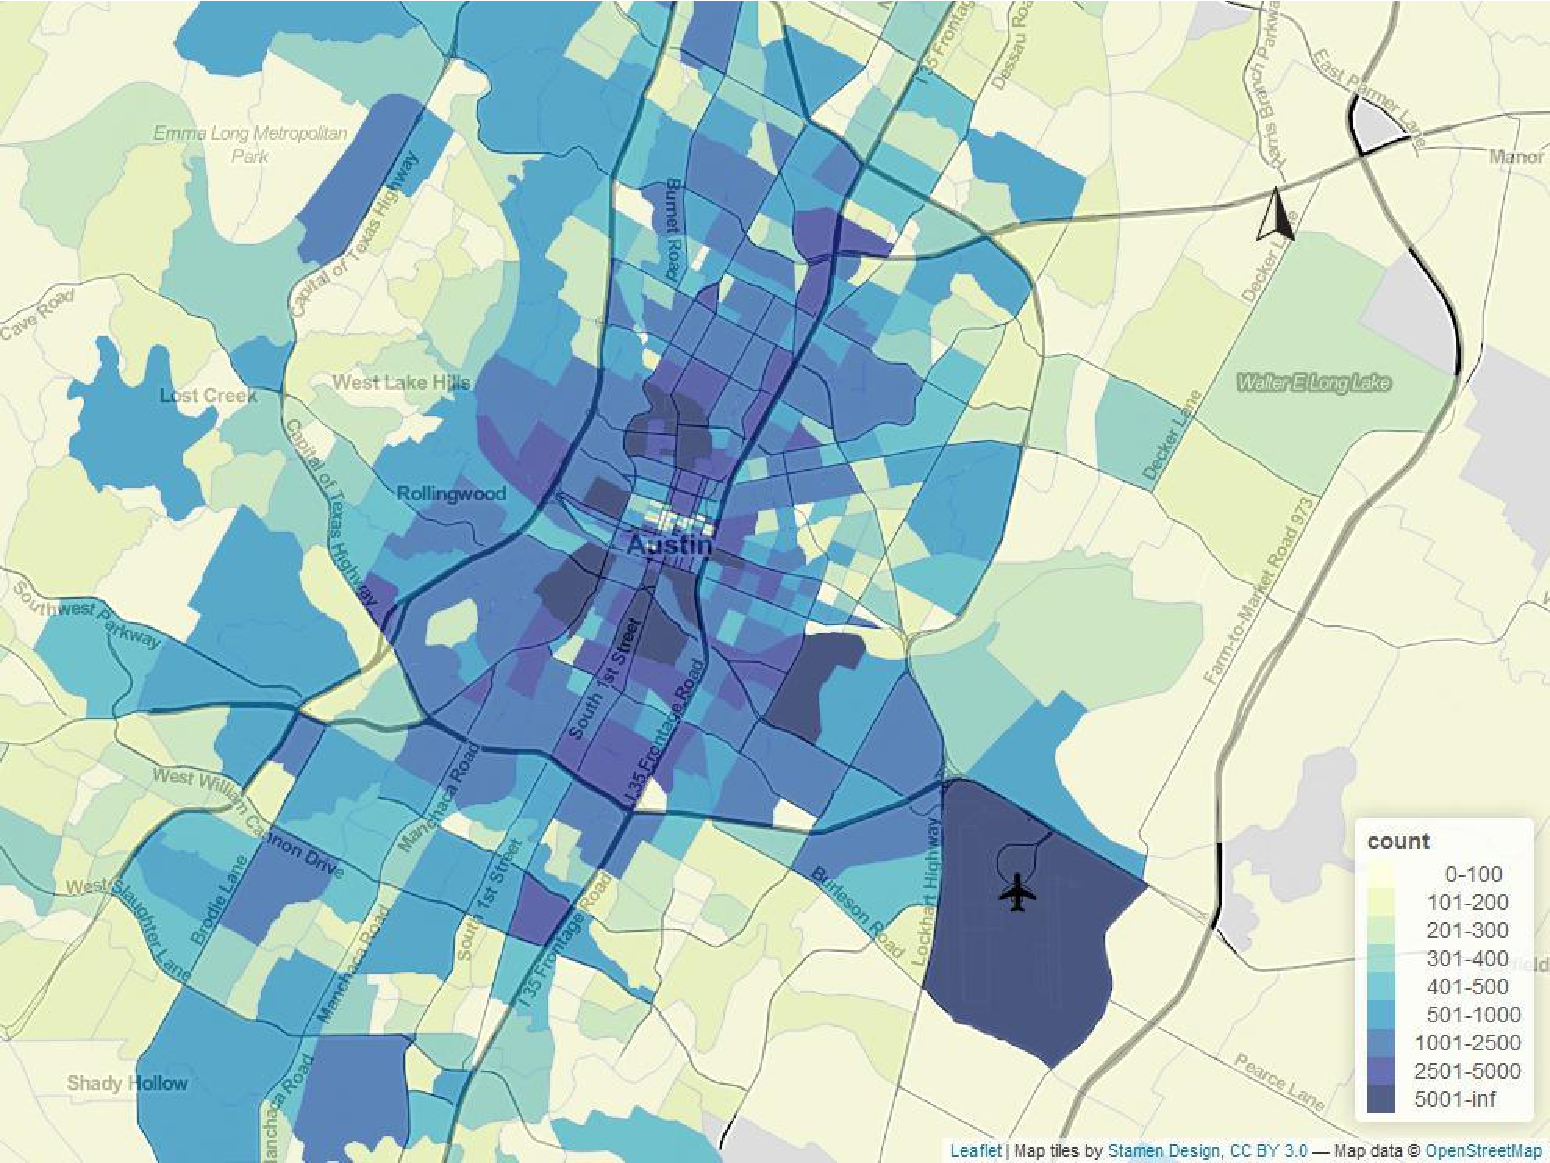
\includegraphics[width=0.7\linewidth]{img/prodhist_spatial.pdf}
        \caption{Counts aggregated by space units}
        \label{fig:prod:spatial}
    \end{subfigure}%
    \caption{Counts of trips marginally aggregated by time and space} 
    \label{fig:prod_spacetime}
\end{figure}

\subsection{Model specification}

\subsubsection{Binary splittings}

We decided to use a binary tree of 5 levels, yielding 32 bins. To choose this bins smartly, we used quantiles of the global productivity distribution to define splitting points in the range (0, 125) which contains 99.98\% of the data\footnote{After examining the data, there are reasons to belief that the top 0.02\% observations come from failures in the data recording system.}. The resulting cutting points are shown in Figure \ref{fig:splits}. While this choice has the undesirable consequence of making our model choice data-dependent, it brings two great benefits:
\begin{itemize}
    \itemsep0em
    \item It naturally uses resolution in regions that had more observations. Alleviating the effects of discretization, and decreasing the need of deeper binary trees.
    \item Unless the local distribution of a vertex dramatically differs from the global distribution, it generates better balanced splits, in the sense that the quantity of observations left and right of each split is more similar; this greatly improved the inference process, since logistic regression does not perform well in highly unbalanced data scenarios.
\end{itemize}
We remark that our decomposition based on quantiles is similar in spirit to the common practice of median splitting used in binary search and kd-trees \citep{bentley-1975}.

\begin{figure}[htb]
    \centering
    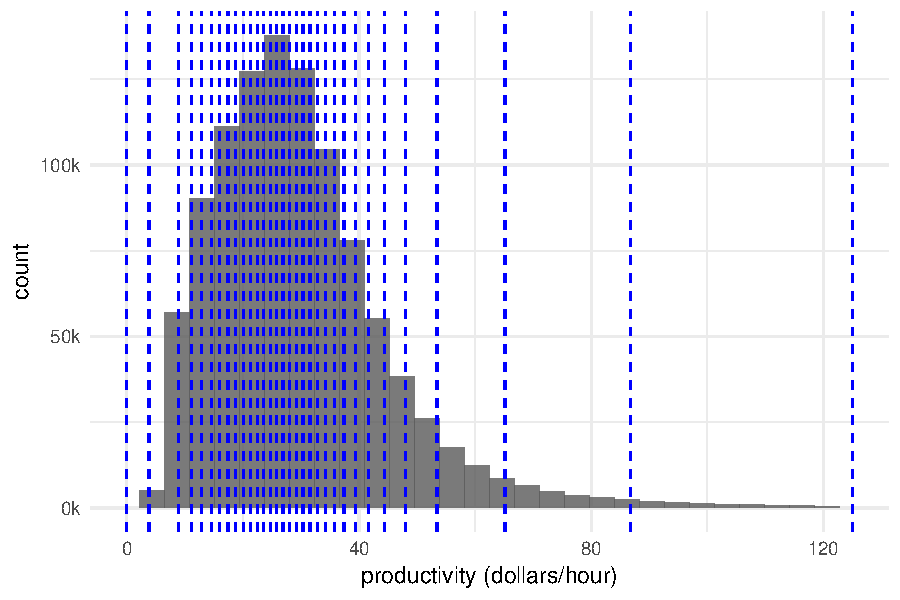
\includegraphics[width=0.55\linewidth]{img/splits.pdf}
    \caption{Vertical dashed lines are the splits used by the binary tree constructed using the quantiles of the global distribution shown in gray.}
    \label{fig:splits}
\end{figure}

\subsubsection{Spatiotemporal total variation with elastic-net penalties}

It is not sensible to equally penalize the total variation in the time and space dimensions. Thus at each split we consider a different pair of $l^1$ and $l^2$-penalties for temporal and spatial dimensions. Thus, the loss function for each split $\gamma$ takes the form
\begin{equation}
\begin{aligned}
\min_{\beta \in \mathbb{R}^{|V|}} & \quad \sum_{v \in V} \left\{ m_v^{(\gamma)} \log(\sigma(\beta_v)) + (m_v^{(\gamma)} - y_v^{(\gamma)})\log(1 - \sigma(\beta_v)) \right\} \\
 & + \sum_{(v,w) \in E_S} \left\{ \lambda_{S,1} \left|\beta_v -\beta_w\right|  
 + \frac{\lambda_{S,2}}{2} \left(\beta_v -\beta_w\right)^2 \right\} \\
 & + \sum_{(v,w) \in E_T} \left\{ \lambda_{T,1} \left|\beta_v -\beta_w\right|  
  + \frac{\lambda_{T,2}}{2} \left(\beta_v -\beta_w\right)^2 \right\}
\end{aligned}
\label{eq:exprmntobj} 
\end{equation}
with $\sigma(x) := (1 + \exp(-x))^{-1}$ the sigmoid function. Since we are using a 5-depth binary decomposition, we fit in parallel a total of 32 models with the optimization problem defined by \eqref{eq:exprmntobj}.

\subsubsection{Hyper-parameter tuning with Bayesian Optimization}

We used 5-fold cross-validation to choose the best set of hyperparameters $\theta=(\lambda_1, \lambda_2, \eta_1, \eta_2)$. Since grid search hyper-parameter tuning is already costly for a 4-dimensional space, we used Bayesian Optimization \citep{snoek-etal-2012} with a Gaussian Process model to guide the search. The Gaussian Process procedure  assumes that the finite-dimensional distributions of the out-of-sample negative loglikelihood $(l_1,...,l_n)$ corresponding to hyperparameters $(\theta_1,...,\theta_n)$ have multivariate normal distribution
$$
(l_1,...,l_n)  \sim \mathrm{Normal}(0, K), 
$$
with $K:=(K_{ij})_{i,j=1}^n$ some Kernel matrix. We chose the Gaussian kernel $K_{ij}=\exp(-\lVert \theta_i - \theta_j\rVert^2_2/2)$.

The idea of Bayesian optimization is that every time we obtain an estimate of the out-of-sample loss $l_i=l(\hat{\beta}_i; \theta_i)$ using cross validation, we can update our knowledge about the predictive distribution of $l_* = l(\hat{\beta}_*; \theta_*)$ for an untested $\theta_*$. We proceed in generations; in each step, we use the current estimate of the predictive distribution to generate a sample of hyperparameters with small predicted out-of-sample loss. After we repeat the inference procedures with the new combinations of hyperparameters and estimate the new out-of-sample losses, we update our posterior predictive using Bayesian inference. In our case, 10 generations of size 16 worked well. Note that the procedures within each generation can be embarrassingly parallelized. We refer the reader to \citep{shahriari-etal-2016} for a broader explanation on Bayesian optimization.

\subsection{Results}

\subsubsection{Overview of the inference results}

Figure \ref{fig:spacetime-densities} shows the estimated densities. We include five locations that have distinct characteristics that highlight different aspects of the inference. Table \ref{tbl:locations} shows a summary description of the selected sites. We choose central areas with high and low demand (university, downtown, Red River \& 12th), two suburbs with different trip count (Domain and Pflugerville), and the airport area. We show the estimates in intervals of 12 hours during 8am and 8pm. Several interesting qualitative remarks are readily available:

\begin{itemize}
    \item \textit{Not all days are equal}. When considering whether we should include a time observation for each time of the week or just each day, we suspected that each day had slightly different dynamics. We see that in a typical Wednesday 8am, most locations have a density close the global mean, whereas in a typical weekend morning, the locations in the central area (University, downtown, Red River \& 12th) have higher productivity. Mondays and Fridays have also higher productivity than the rest of business days. 
    \item \textit{Smoothing is turned on}. With a few exceptions, the estimates of the locations we chose in central Austin (University, downtown and Red river \& 12th). This is particularly remarkable since Red river had almost no observations. It is also evident regions without observations are not pull towards the global mean, since the region behaves very differently from the global mean.
    \item \textit{We recover periodic patterns}. In our analysis, we chose not to create edges between different days of the week at the same time of the day (e.g., there is no direct edge between a Monday 8pm and Tuesday 8pm). Nevertheless, we do observe periodic patterns for some locations, notably, the airport. Every morning around 8am its distribution is close the global mean, however, every afternoon it is shifted downwards.
\end{itemize}


\begin{table}[htb]
    \centering
    \begin{tabular}{c|p{10cm}}
        \textbf{Location} & \textbf{Description} \\ \hline
        Airport &  Austin-Bergstrom International Airport. It is the single TAZ with more trips. \\ \hline
        The Domain & Office, retail, and residential center outside central Austin. It has medium-low density of trips. \\ \hline
        Pflugerville & Large suburban area located far from the central area. It has low count of trips.  \\ \hline
        University & The University of Texas at Austin main campus. It is located adjacent to central business district. It has a high number of trips.  \\ \hline
        Downtown &  Central business district. It comprises several small TAZs with a large number of trip counts. An arbitrary TAZ was selected in the intersection of 6th \& Guadalupe St. \\ \hline
        Red River \& 12th & Red River is a popular street with restaurants and bars near the central area. However, the exact TAZ that contains the intersection with 12th has a very low trip count.
    \end{tabular}
    \caption{Locations used in figure \ref{fig:spacetime-densities} for comparison of density estimates}
    \label{tbl:locations}
\end{table}

\begin{figure}[htb]
    \centering
    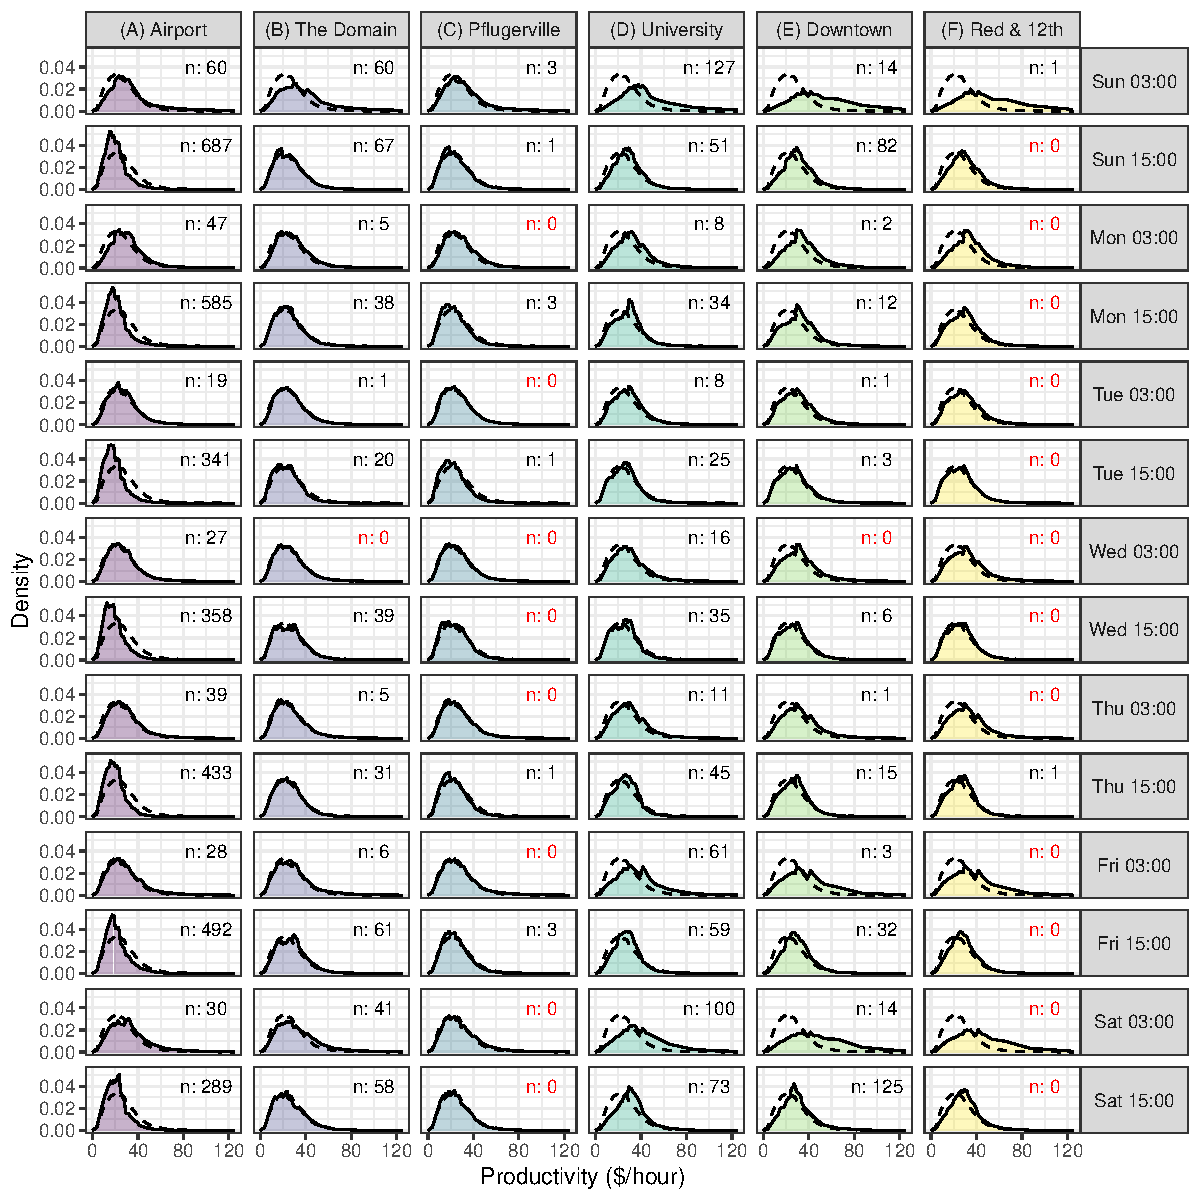
\includegraphics[width=0.98\linewidth]{img/densities_spacetime.pdf}
    \caption{Driver Productivity by Time and Location. The global distribution is shown (dashed); the number of observed data points in the corresponding node of the graph is shown in the upright corner of each density plot (n). Time is shown every 12 hours.}
    \label{fig:spacetime-densities}
\end{figure} 


To further evaluate the time smoothness of the estimates, we show in figure \ref{fig:airport-densities} the estimates at the airport area in intervals of two hours. This completes the picture of the periodic pattern found in figure \ref{fig:spacetime-densities}, since it shows a smooth transition between mornings, when the distribution of productivity is closer to the global mean, to afternoons, when it is smaller. It is interesting to mention that while other locations showed a very different distribution during weekends and business days, the airport is more similar every day.



\begin{figure}[htb]
    \centering
    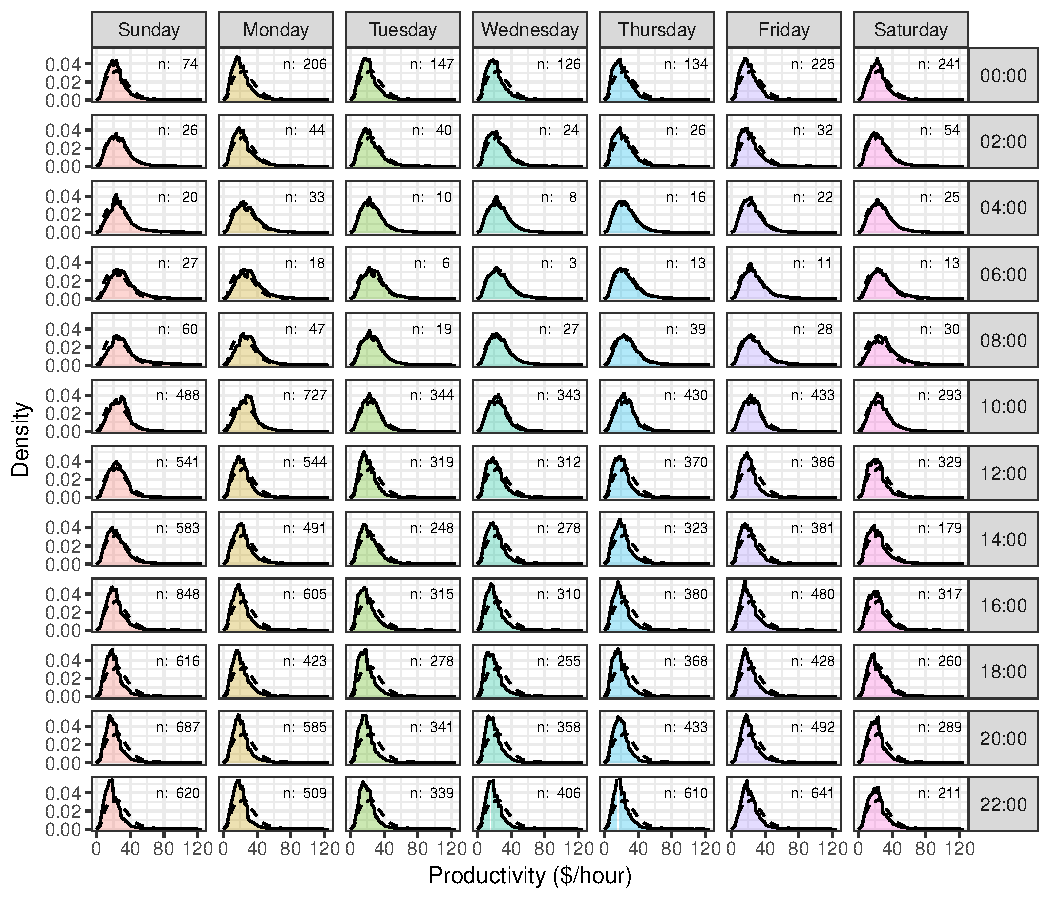
\includegraphics[width=0.98\linewidth]{img/densities_airport.pdf}
    \caption{Driver Productivity of the Airport TAZ. The global distribution (dashed); the number of arriving flights during the observation period (a); the number of departing flights (d); the number of observations in the dataset (n). Time is shown every two hours for the seven days of the week.}
    \label{fig:airport-densities}
\end{figure}


\subsubsection{Investigating driver productivity}

 We present a list of interesting scientific enquiries that can be answered using the full distributions of productivity at each location and time. 
 
 \begin{enumerate}
     \item \textit{Tail probabilities}: What is the probability of not exceeding a specific salary? We compare to standardized living wages in Travis County, TX \citep{nadeau-2017}. 
     \item \textit{Quantiles}: How many dollars per hour constitute the $\alpha$-level quantile? We are interested in assessing the risk of the $\alpha$\% worst performers.
 \end{enumerate}
 
 We provide answers to some of these questions in this section; the others are included in the supplemental material. 

{\bfseries \itshape Tail probabilities: the risk of not attaining a living wage}. We seek to estimate the probability that a driver will obtain a minimum living salary. Table \ref{tbl:livingwages} shows estimated living wages for families living in Austin in 2017 \citep{nadeau-2017}. 

To these wages, we must add the activity-specific additional costs such as the fixed fee of \$0.99 charged per trip charged by RideAustin as well as car maintenance, which on average lies around \$6.40 hourly pretax and \$4.78 hourly after tax deductions \citep{mishel-2018} \citep{hall-etal-2016}. Since a driver completes more than one trip per hour, we rounded up the costs to \$6.00. The final reference values including costs are also presented in table \ref{tbl:livingwages}.

\begin{table}[htb]
    \centering
    \small
    \begin{tabular}{l|l|l|l|l}
        % \hline
        \textbf{\# adults} & 1 adult &  2 adults & 2 adults (1 working) & 1 adult  \\ % \hline
        \textbf{\# children} & 0 children  &   2 children & 2 children & 2 children  \\
       \hline
        \textbf{living wage} & \$12.56  & \$15.64 & \$26.73 & \$28.74  \\ 
        \textbf{living wage+costs} & \$18.56  & \$21.64 & \$32.73 & \$34.74  \\ 
        % \hline
    \end{tabular}
    \caption{Hourly living wages in Austin, TX \citep{nadeau-2017}. The costs are calculated using the \$0.99 RideAustin fee per ride and an estimation of \$4.78 hourly maintenance cost after tax deductions \citep{mishel-2018}.}
    \label{tbl:livingwages}
\end{table}

Figure \ref{fig:wages} shows the results for the case of two working adults with two children (\$21.64) for different times of the week and regions of the city. The remaining cases are included in appendix \ref{appendix:maps_livingwages}. We observe that during a Sunday morning when the traffic is low and there is a high demand (\textit{c.f.} figure \ref{fig:prod:timely}) the probability of exceeding the living wage is close to 90\% near downtown and it decreases to around 70\% as a driver lies farther away from central Austin. In contrast, during at Monday 6pm, with moderate demand but high traffic, the probability ranges from 40\% to 60\%, being worst at the airport. These suggests that drivers are at a high risk of not making a living wage.

\begin{figure}[htb]
    \centering
    \begin{minipage}[t]{0.48\linewidth}
        \centering
        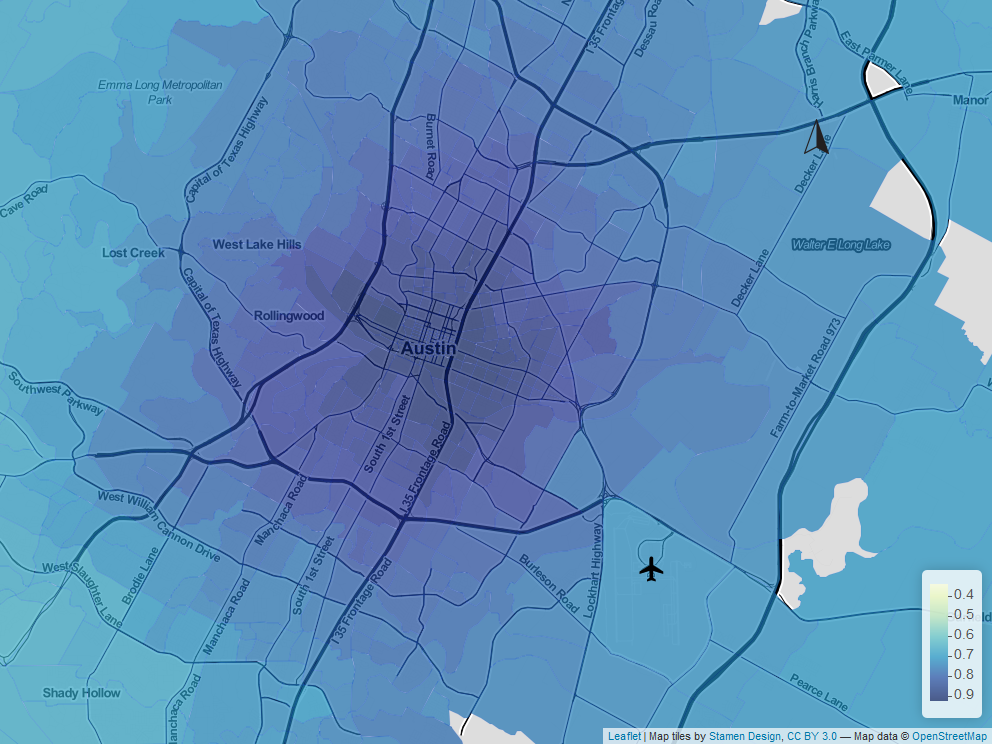
\includegraphics[width=\linewidth]{img/tailprob_21_64__9.png}
        \subcaption{Sunday 8am (weekend low traffic)}
        \label{fig:wages:a}
    \end{minipage}
    \begin{minipage}[t]{0.48\linewidth}
        \centering
        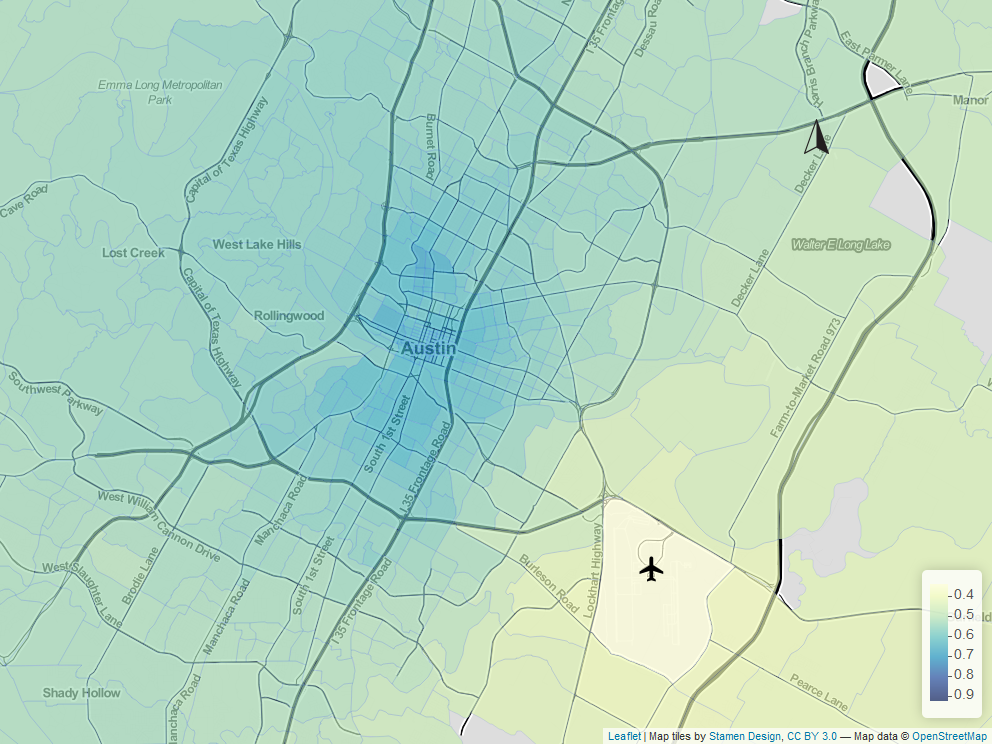
\includegraphics[width=\linewidth]{img/tailprob_21_64__43.png}
        \subcaption{Monday 6pm (weekday rush hour)}
        \label{fig:wages:b}
    \end{minipage}\hfill
    \begin{minipage}[t]{.48\linewidth}
        \centering
        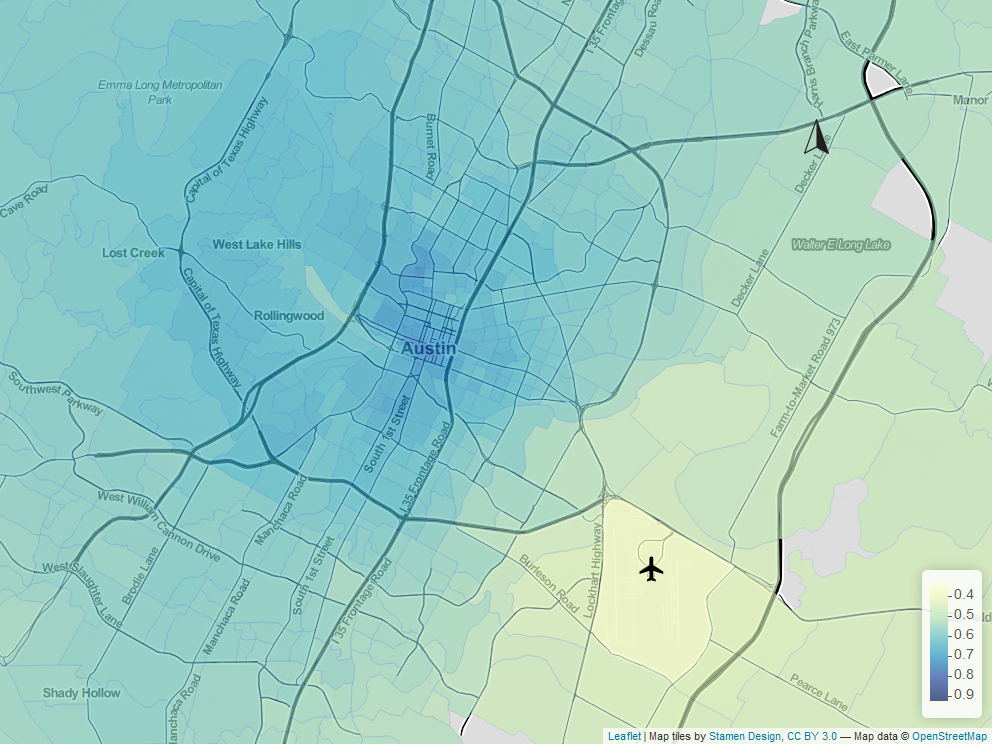
\includegraphics[width=\linewidth]{img/tailprob_21_64__142.png}
        \subcaption{Friday 9pm (weekday social mild traffic)}
        \label{fig:wages:c}
    \end{minipage}
    \begin{minipage}[t]{0.48\linewidth}
        \centering
        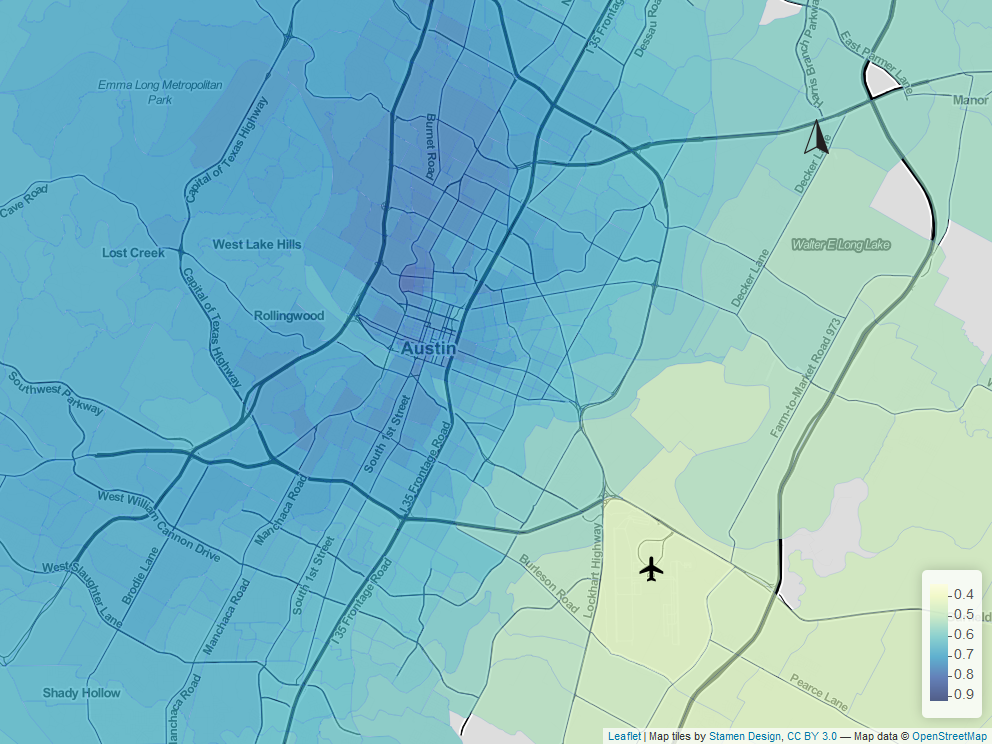
\includegraphics[width=\linewidth]{img/tailprob_21_64__168.png}
        \subcaption{Saturday 11pm (weekend social low traffic)}
        \label{fig:wages:d}
    \end{minipage}
    \caption{Probability of exceeding \$21.64 in the next hour given a current location (living wage with costs for two working adults with two children).}
    \label{fig:wages}
\end{figure}

{\bfseries\itshape Quantiles: How bad are the worst performers doing?}. As a company seeking to guarantee the well-being of its workers, it makes sense to target the population at specific levels of risk. One may ask, What is the expected income of the lowest $100 \alpha\%$ percent? That is, for each location and time, we seek to find the quantity
$$
q_\alpha := \min_{q\in[0,125]}P(\mathtt{productivity} > q) > \alpha
$$
Usual interesting values for $\alpha$ are $\{0.1, 0.25, 0.5, 0.75, 0.9\}$. The case $\alpha = 0.1$ is shown in figure \ref{fig:quantiles:0.1}, the rest are included in appendix \ref{appendix:quantiles}. We can see that in a typical Monday 6pm, the rush hour, the lowest $10\%$ quantile is around $\$12$ to $\$15$, being as low as $\$10$ in the airport area. This result should be contrasted with table \ref{tbl:livingwages}, which states that a living wage of a single working adult with no children is above $\$18$. The highest value is attained around the central part of the city during weekend mornings when there is low traffic and high demand (\textit{c.f.} figure \ref{fig:prod:timely}).

\begin{figure}[htb]
    \centering
    \begin{minipage}[t]{0.48\linewidth}
        \centering
        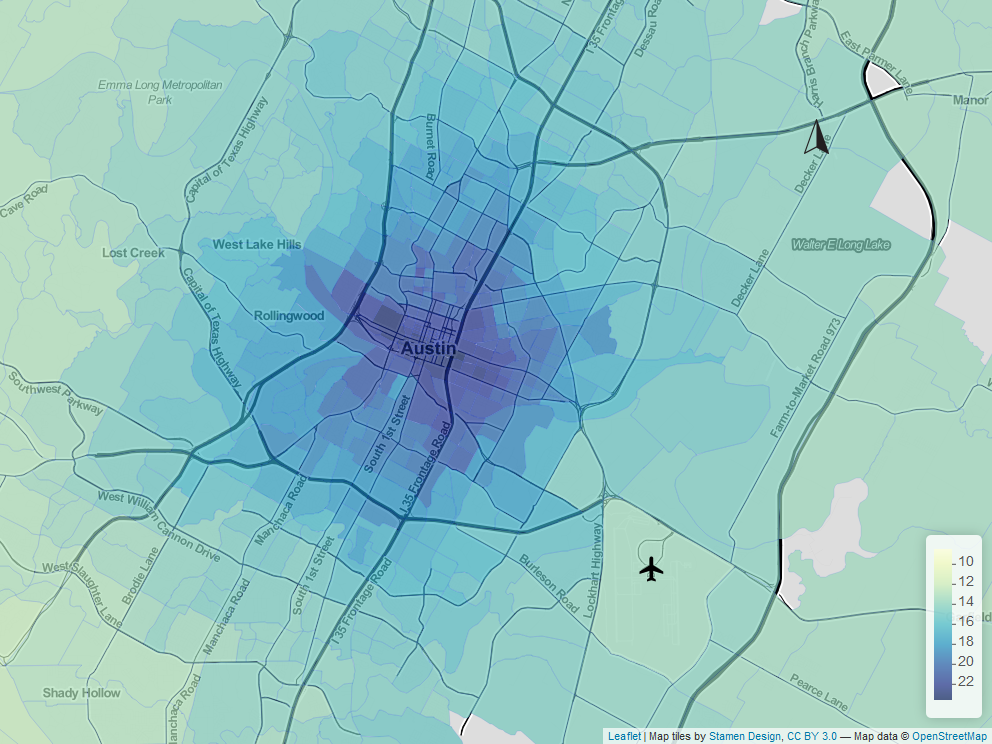
\includegraphics[width=\linewidth]{img/quantile_9_1.png}
        \subcaption{Sunday 8am (weekend low traffic)}
        \label{fig:quantiles:0.1:a}
    \end{minipage}
    \begin{minipage}[t]{0.48\linewidth}
        \centering
        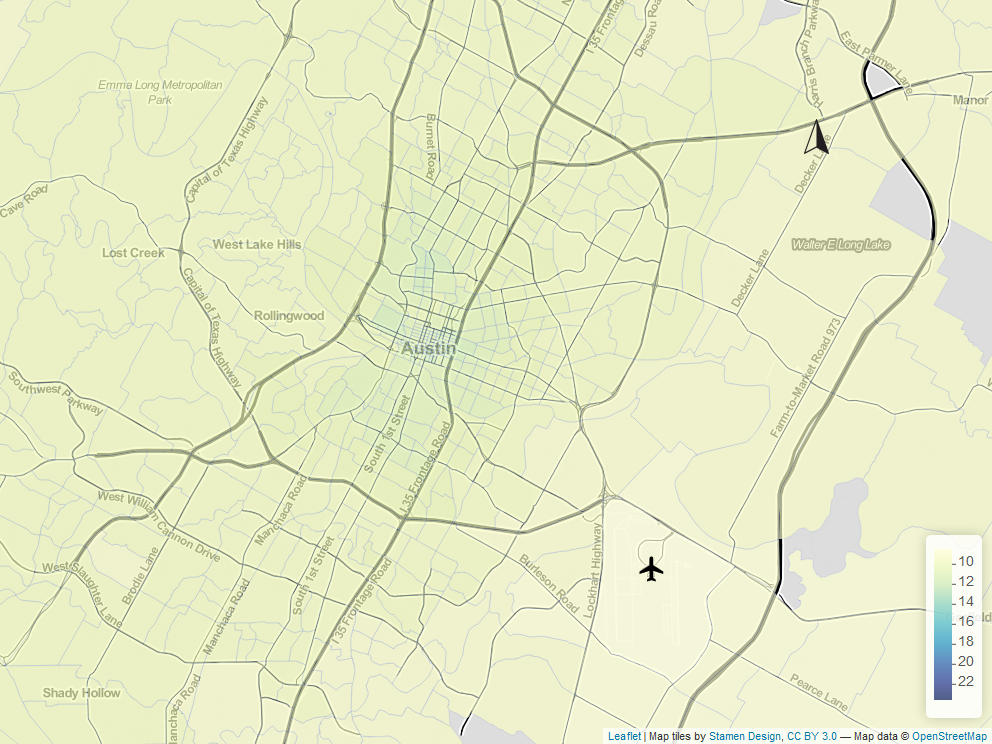
\includegraphics[width=\linewidth]{img/quantile_43_1.png}
        \subcaption{Monday 6pm (weekday rush hour)}
        \label{fig:quantiles:0.1:b}
    \end{minipage}\hfill
    \begin{minipage}[t]{.48\linewidth}
        \centering
        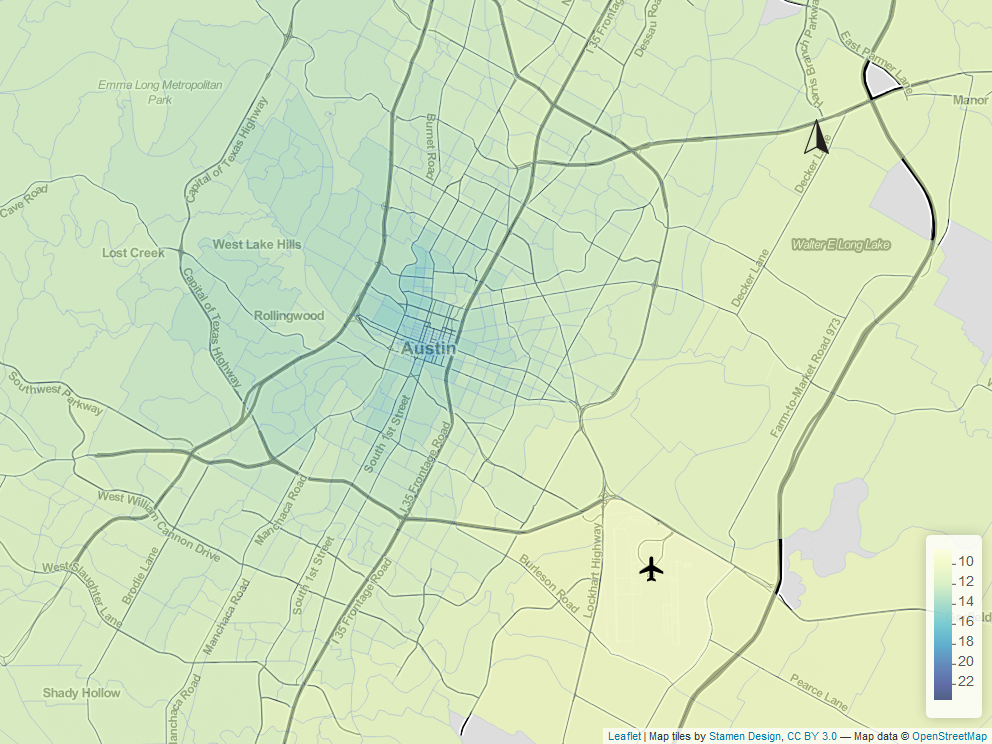
\includegraphics[width=\linewidth]{img/quantile_142_1.png}
        \subcaption{Friday 9pm (weekday social mild traffic)}
        \label{fig:quantiles:0.1:c}
    \end{minipage}
    \begin{minipage}[t]{0.48\linewidth}
        \centering
        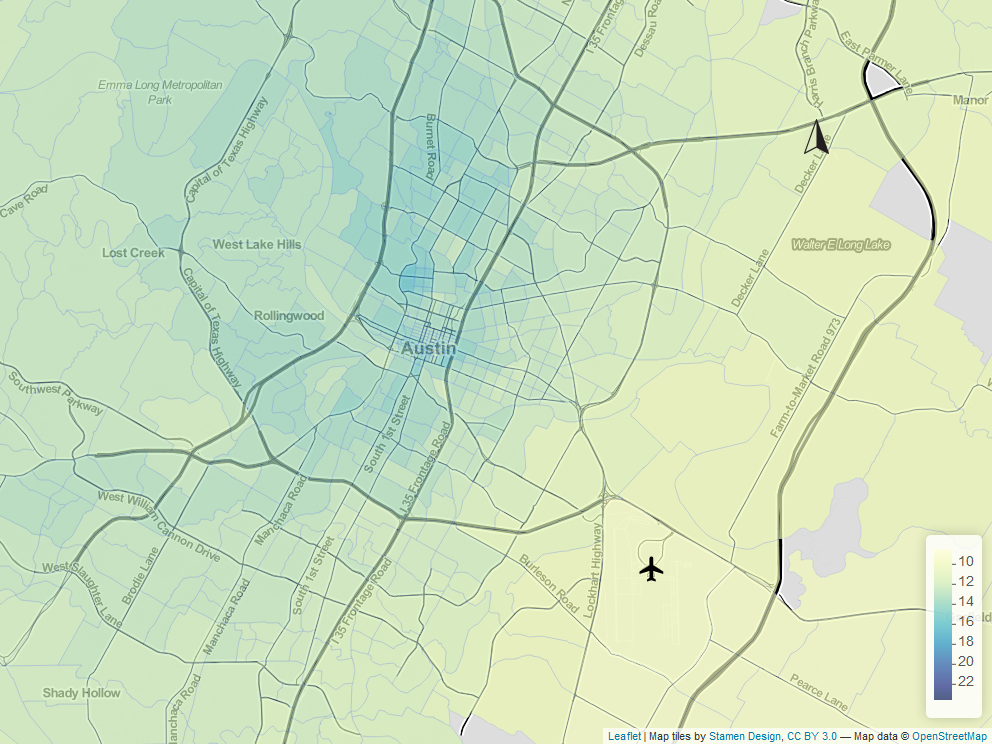
\includegraphics[width=\linewidth]{img/quantile_168_1.png}
        \subcaption{Saturday 11pm (weekend social low traffic)}
        \label{fig:quantiles:0.1:d}
    \end{minipage}
    \caption{Lower 10\% quantile of productivity for different times and locations.}
    \label{fig:quantiles:0.1}
\end{figure}

Given that we have quantiles, a natural measure of spread to consider is the inter-quartile range
$$
\text{IQR} = q_{0.75} - q_{0.25}.
$$
This quantity is preferred over standard deviation for skewed distributions such as our measure of productivity. Figure \ref{fig:iqr} shows the IQR for different times and locations. It must be pointed out that this is measure of spread does not take into account the uncertainty arising from the estimation procedure, but only the variability in the estimated densities. Figure \ref{fig:iqr} complements our previous inquiry using tail probabilities and quantiles in the sense that it shows that the highest reward observed Sunday 8am when there's high demand and low traffic, comes accompanied by higher variability, and not only a shift in location.

\begin{figure}[htb]
    \centering
    \begin{minipage}[t]{0.48\linewidth}
        \centering
        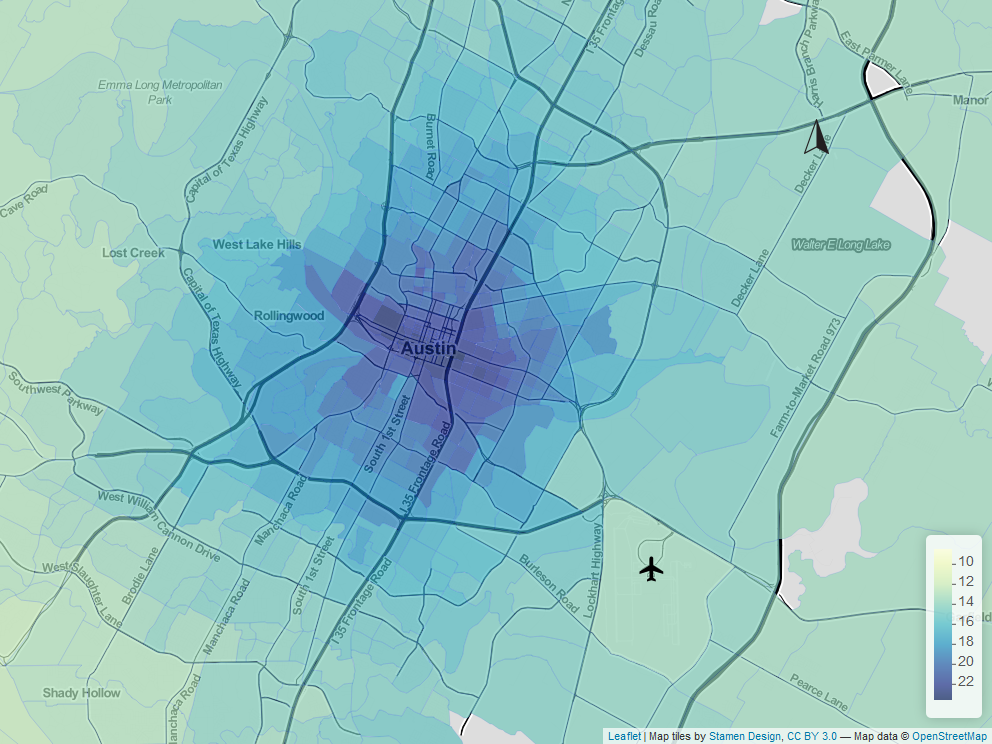
\includegraphics[width=\linewidth]{img/quantile_9_1.png}
        \subcaption{Sunday 8am (weekend low traffic)}
        \label{fig:iqr:a}
    \end{minipage}
    \begin{minipage}[t]{0.48\linewidth}
        \centering
        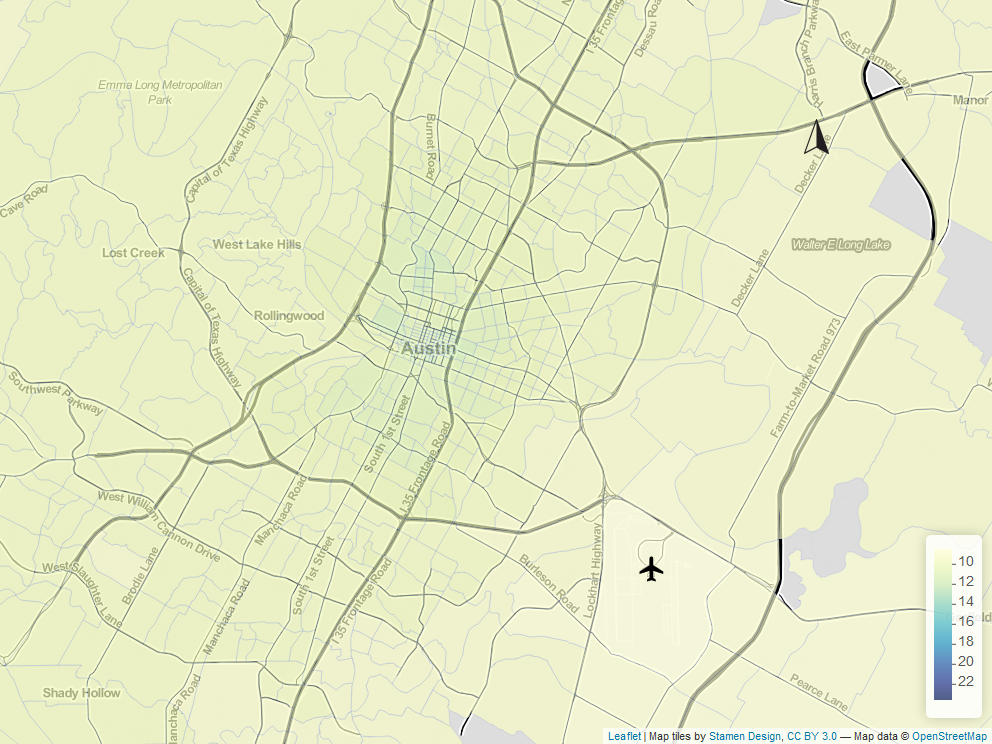
\includegraphics[width=\linewidth]{img/quantile_43_1.png}
        \subcaption{Monday 6pm (weekday rush hour)}
        \label{fig:iqr:b}
    \end{minipage}\hfill
    \begin{minipage}[t]{.48\linewidth}
        \centering
        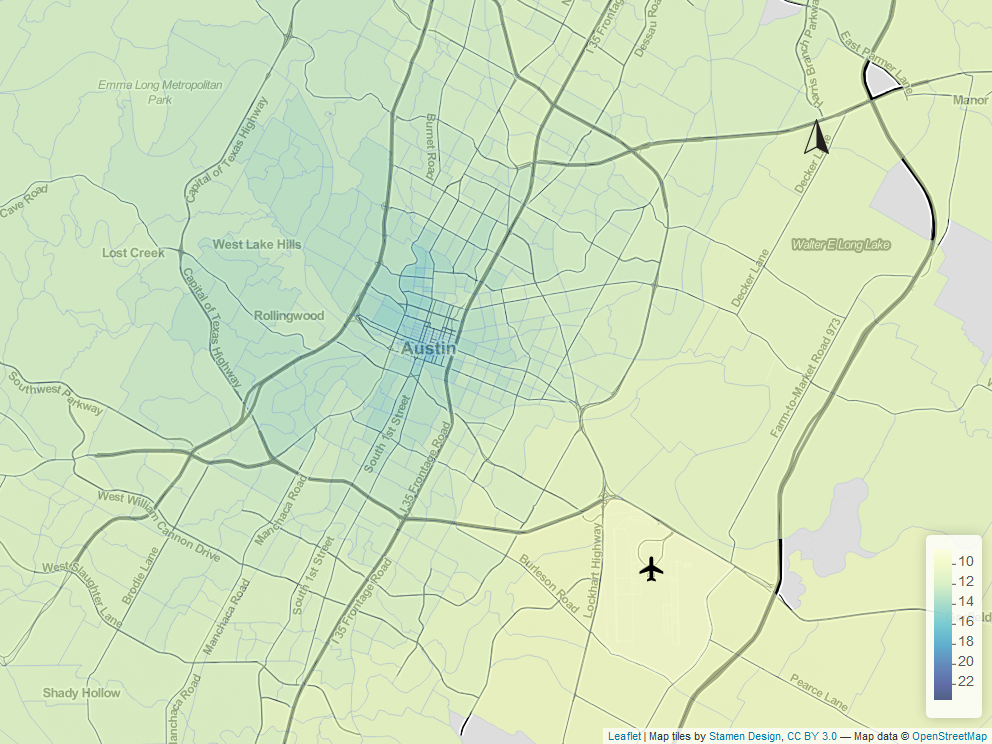
\includegraphics[width=\linewidth]{img/quantile_142_1.png}
        \subcaption{Friday 9pm (weekday social mild traffic)}
        \label{fig:iqr:c}
    \end{minipage}
    \begin{minipage}[t]{0.48\linewidth}
        \centering
        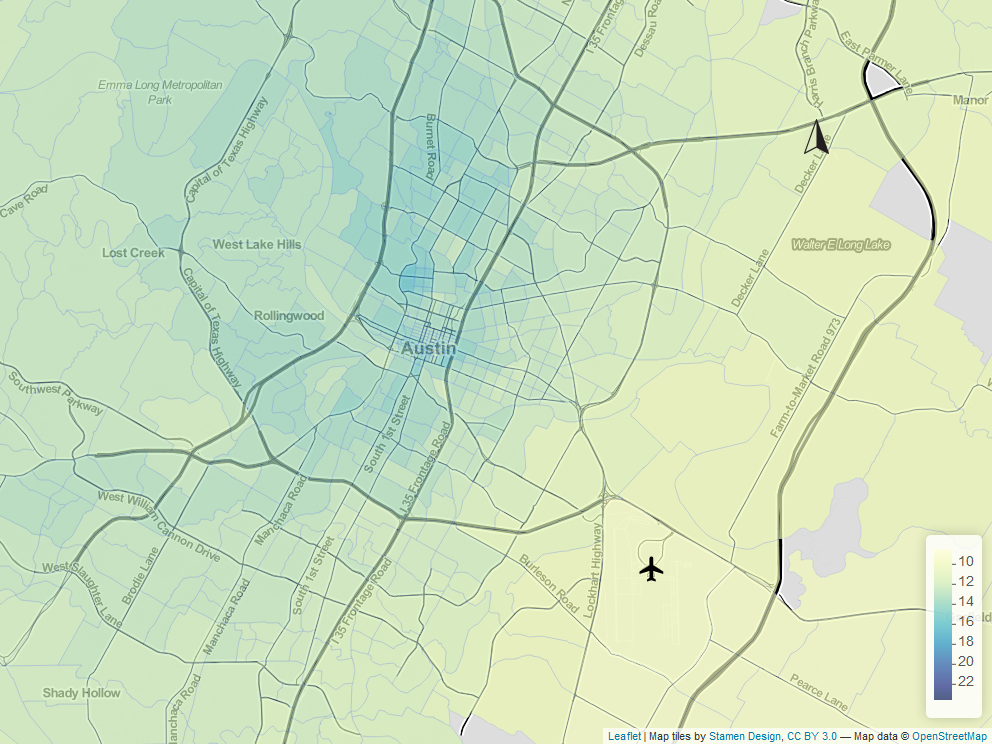
\includegraphics[width=\linewidth]{img/quantile_168_1.png}
        \subcaption{Saturday 11pm (weekend social low traffic)}
        \label{fig:iqr:d}
    \end{minipage}
    \caption{IQR of productivity for different times and locations.}
    \label{fig:iqr}
\end{figure}


\section{Concluding remarks}
\label{sec:conc}


\appendix
% \section{Tail probabilities of not exceeding living wage}
\label{appendix:maps_livingwages}

\begin{figure}[htb]
    \centering
    \begin{minipage}[t]{0.48\linewidth}
        \centering
        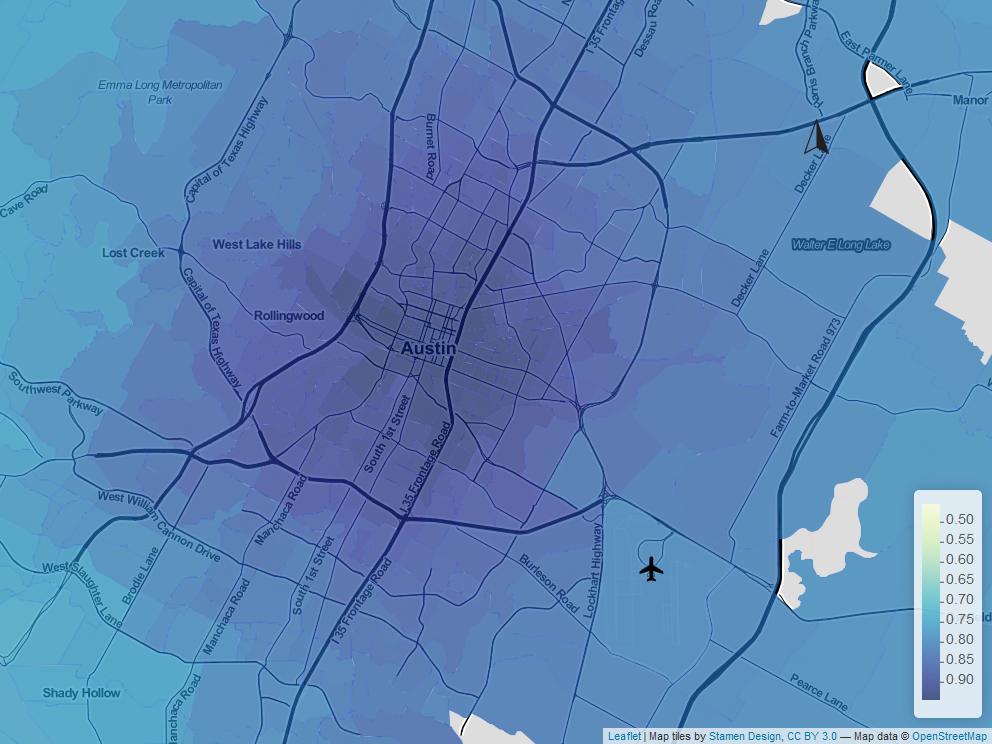
\includegraphics[width=\linewidth]{img/tailprob_18_56__9.png}
        \subcaption{Sunday 8am (weekend low traffic)}
        \label{fig:wages:appendix1:a}
    \end{minipage}
    \begin{minipage}[t]{0.48\linewidth}
        \centering
        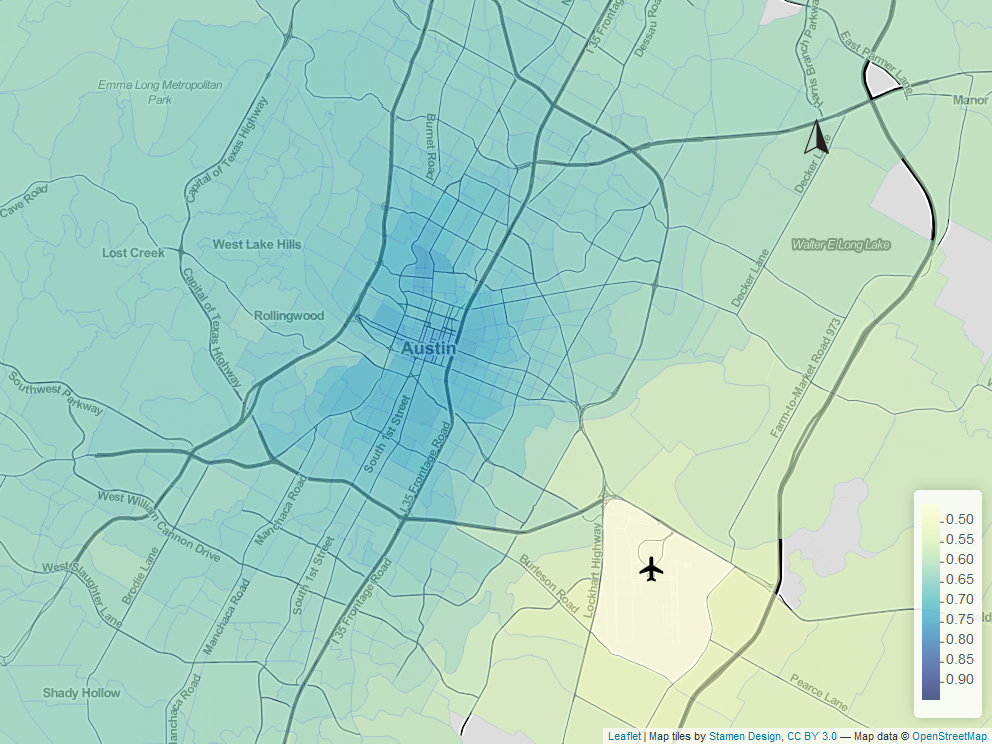
\includegraphics[width=\linewidth]{img/tailprob_18_56__43.png}
        \subcaption{Monday 6pm (weekday rush hour)}
        \label{fig:wages:appendix1:b}
    \end{minipage}\hfill
    \begin{minipage}[t]{.48\linewidth}
        \centering
        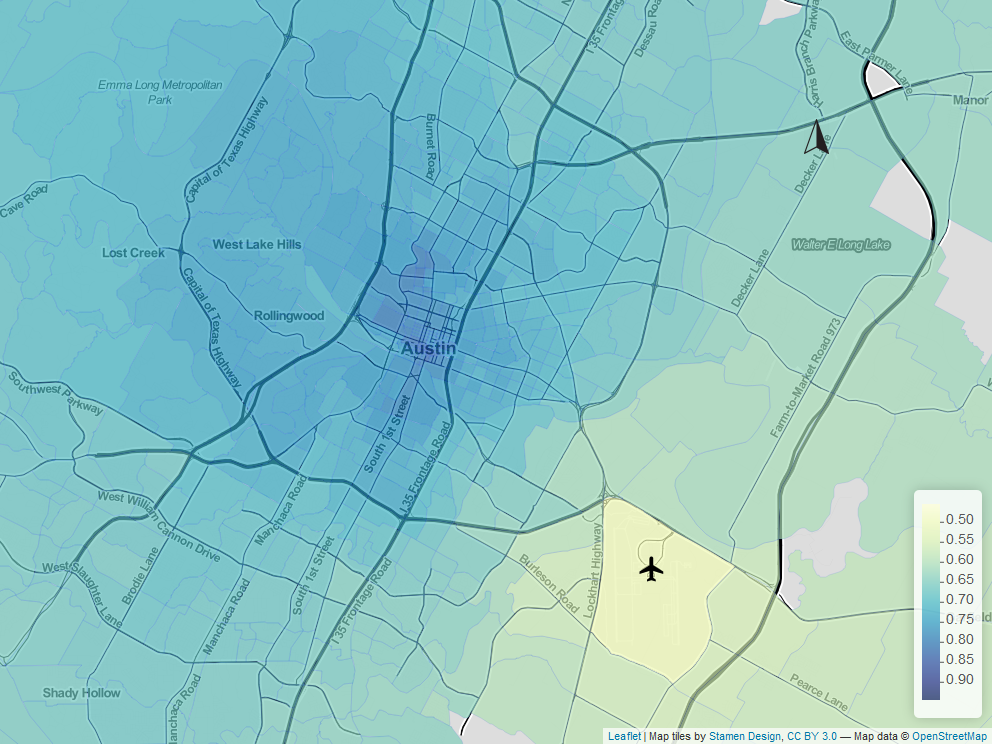
\includegraphics[width=\linewidth]{img/tailprob_18_56__142.png}
        \subcaption{Friday 9pm (weekday social mild traffic)}
        \label{fig:wages:appendix1:c}
    \end{minipage}
    \begin{minipage}[t]{0.48\linewidth}
        \centering
        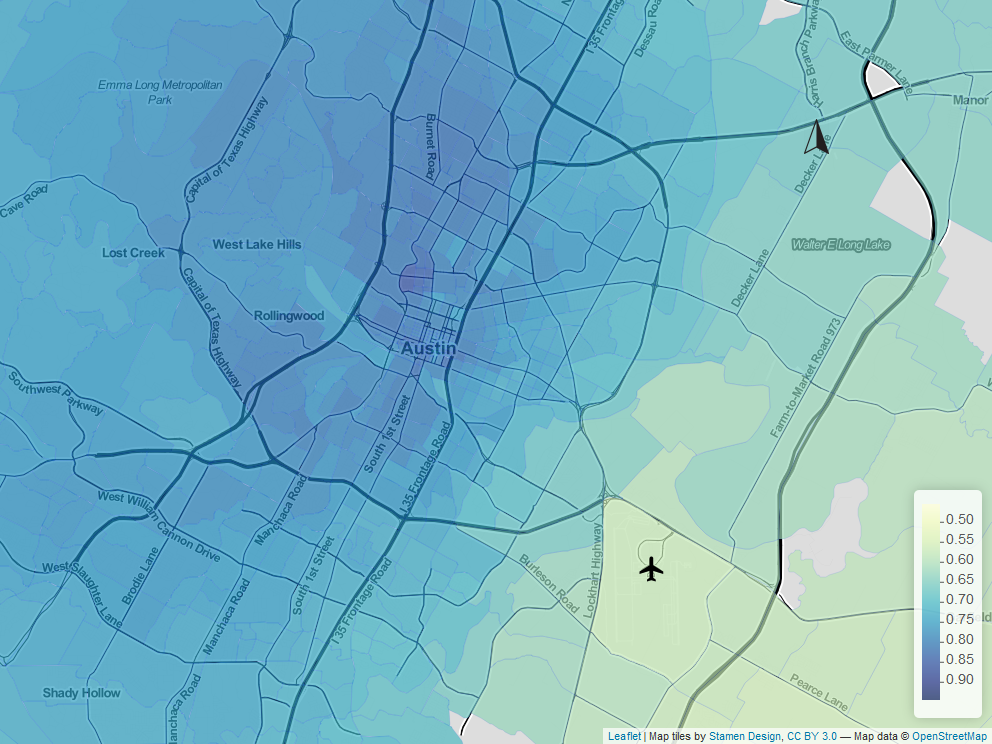
\includegraphics[width=\linewidth]{img/tailprob_18_56__168.png}
        \subcaption{Saturday 11pm (weekend social low traffic)}
        \label{fig:wages:appendix1:d}
    \end{minipage}
    \caption{Probability of exceeding \$18.56 in the next hour given a current location (living wage with costs for one single working adult with no children).}
    \label{fig:wages:appendix1}
\end{figure}


\begin{figure}[htb]
    \centering
    \begin{minipage}[t]{0.48\linewidth}
        \centering
        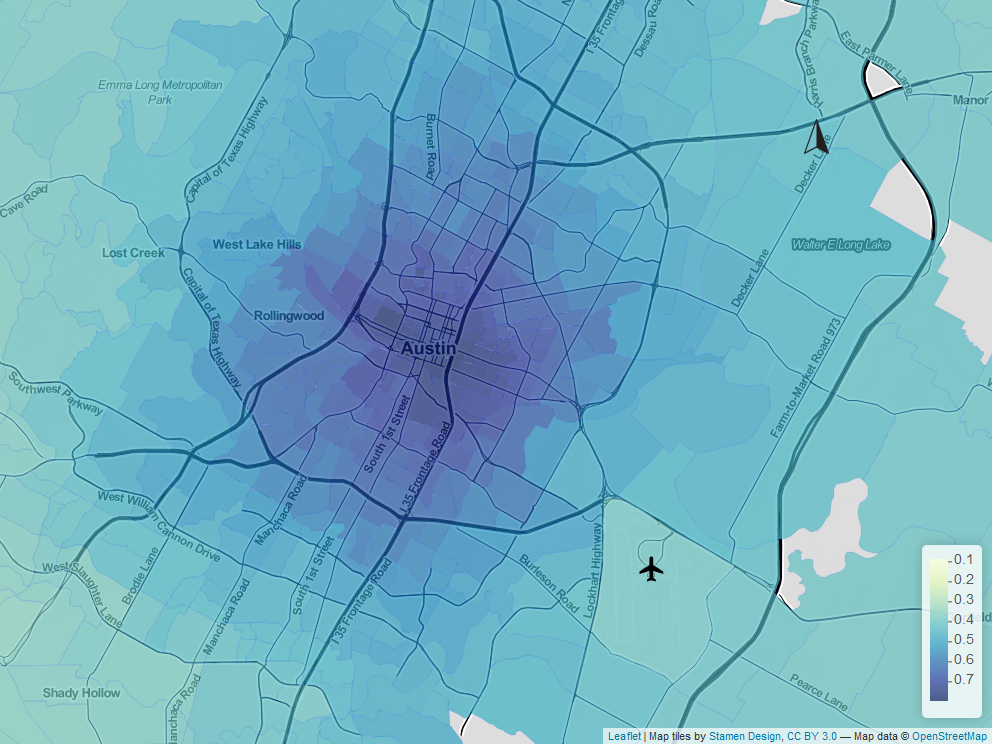
\includegraphics[width=\linewidth]{img/tailprob_32_73__9.png}
        \subcaption{Sunday 8am (weekend low traffic)}
        \label{fig:wages:appendix2:a}
    \end{minipage}
    \begin{minipage}[t]{0.48\linewidth}
        \centering
        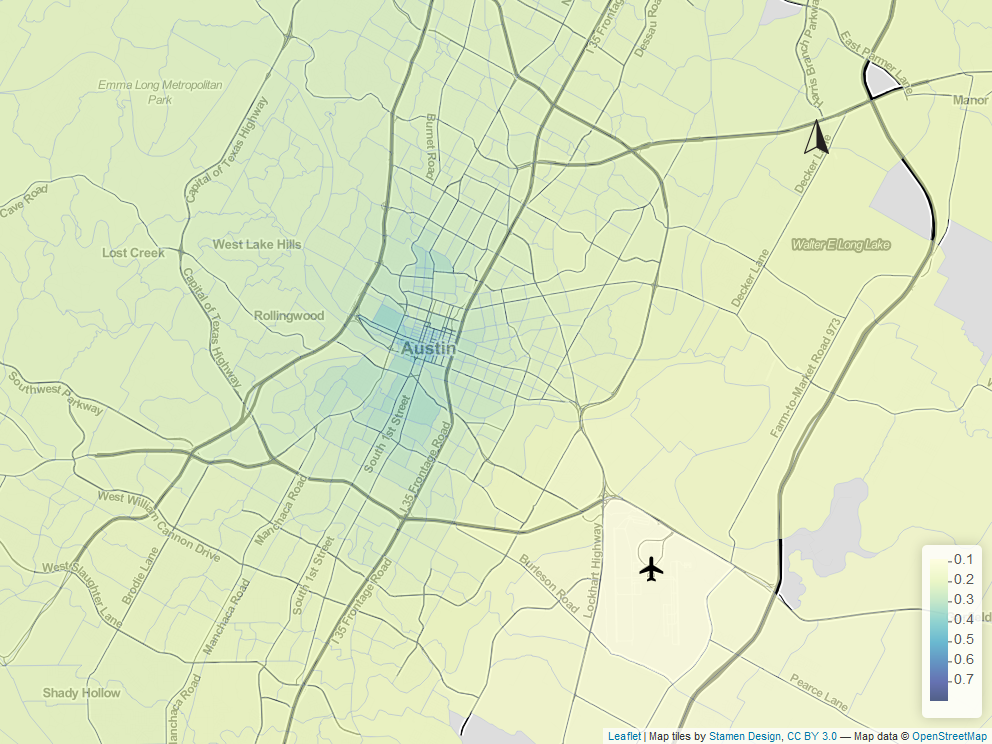
\includegraphics[width=\linewidth]{img/tailprob_32_73__43.png}
        \subcaption{Monday 6pm (weekday rush hour)}
        \label{fig:wages:appendix2:b}
    \end{minipage}\hfill
    \begin{minipage}[t]{.48\linewidth}
        \centering
        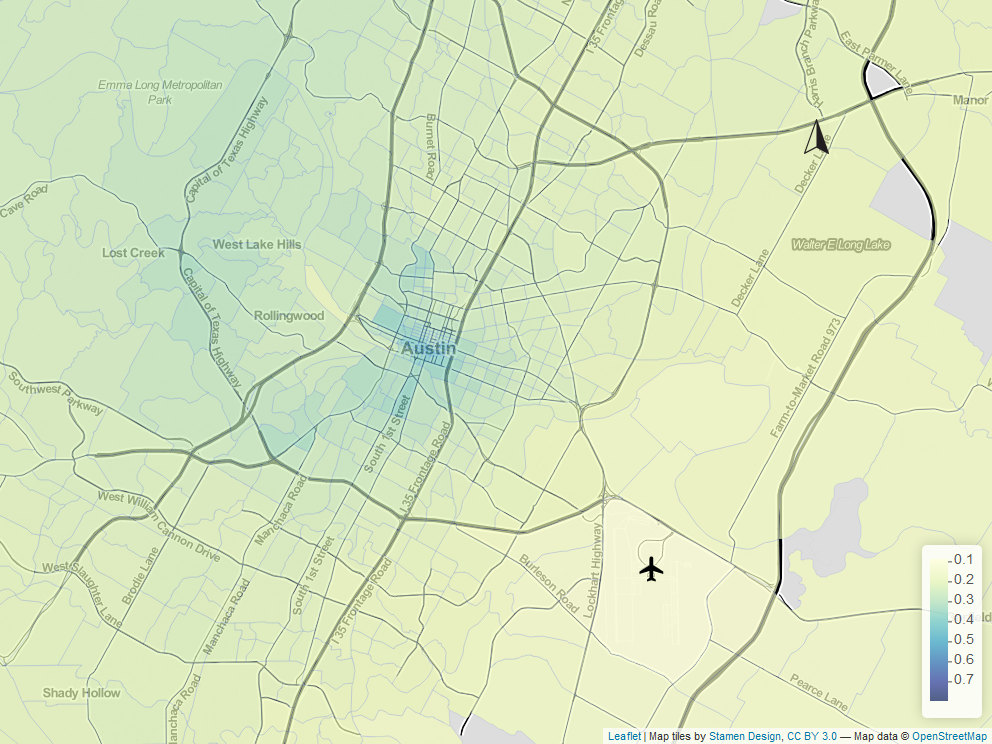
\includegraphics[width=\linewidth]{img/tailprob_32_73__142.png}
        \subcaption{Friday 9pm (weekday social mild traffic)}
        \label{fig:wages:appendix2:c}
    \end{minipage}
    \begin{minipage}[t]{0.48\linewidth}
        \centering
        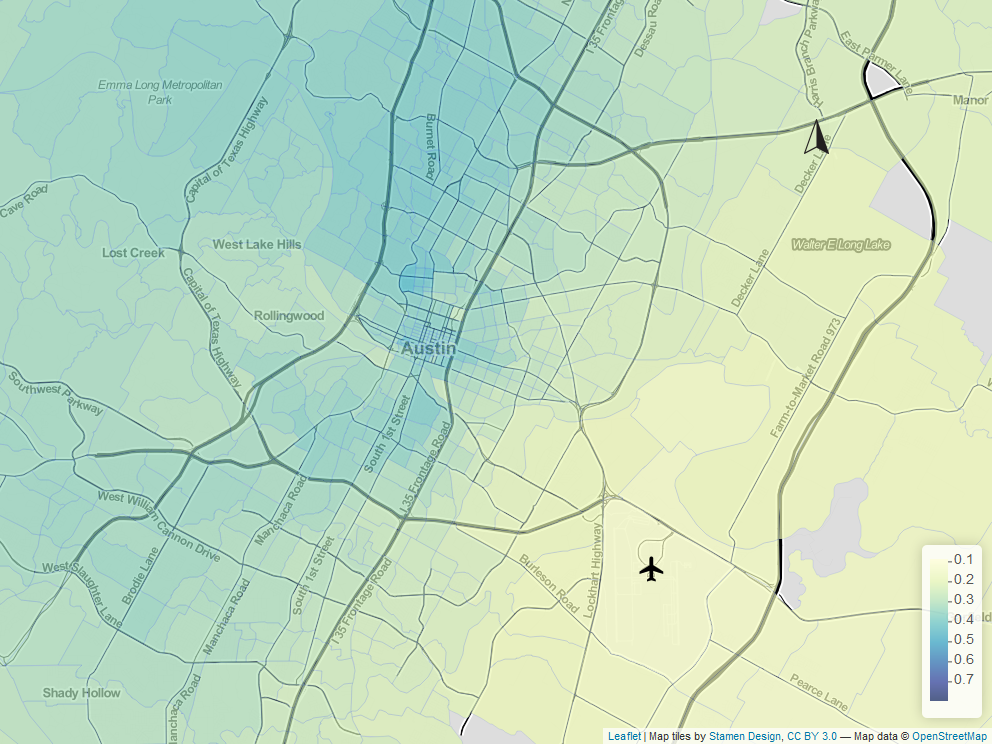
\includegraphics[width=\linewidth]{img/tailprob_32_73__168.png}
        \subcaption{Saturday 11pm (weekend social low traffic)}
        \label{fig:wages:appendix2:d}
    \end{minipage}
    \caption{Probability of exceeding \$32.73 in the next hour given a current location (living wage with costs for two adults, one working, and two children).}
    \label{fig:wages:appendix2}
\end{figure}


\begin{figure}[htb]
    \centering
    \begin{minipage}[t]{0.48\linewidth}
        \centering
        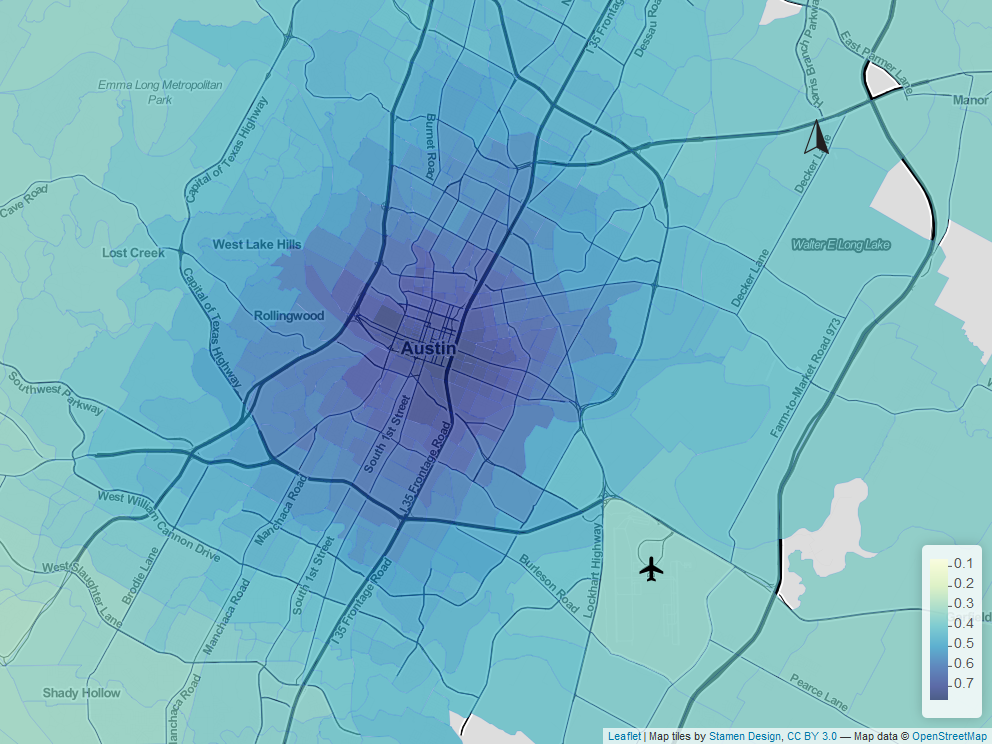
\includegraphics[width=\linewidth]{img/tailprob_34_74__9.png}
        \subcaption{Sunday 8am (weekend low traffic)}
        \label{fig:wages:appendix3:a}
    \end{minipage}
    \begin{minipage}[t]{0.48\linewidth}
        \centering
        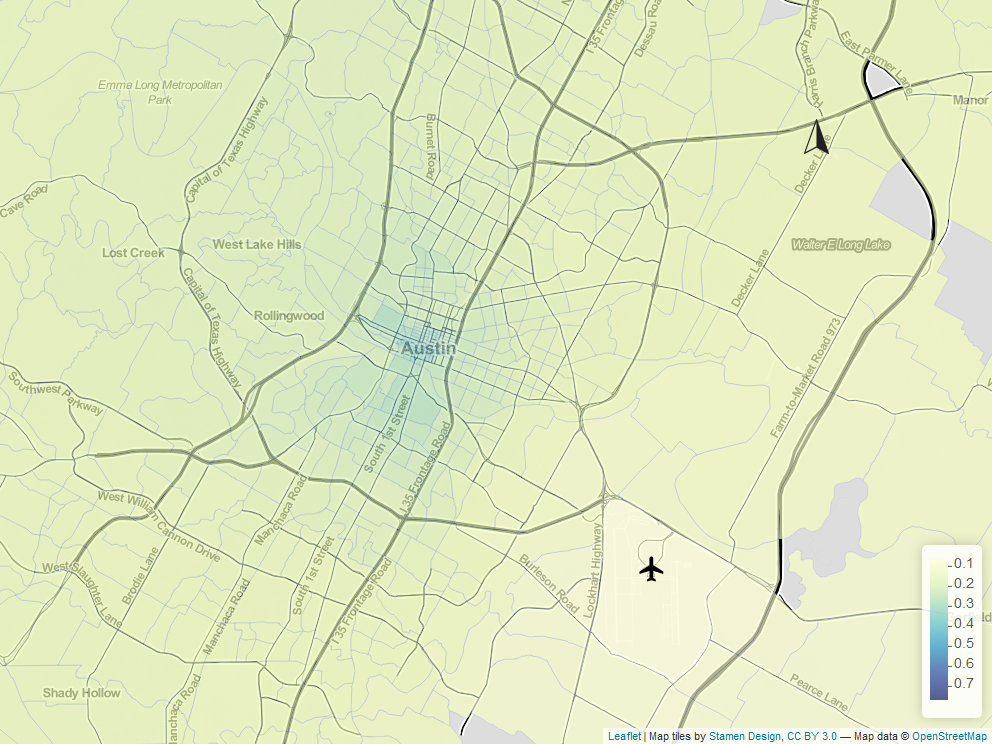
\includegraphics[width=\linewidth]{img/tailprob_34_74__43.png}
        \subcaption{Monday 6pm (weekday rush hour)}
        \label{fig:wages:appendix3:b}
    \end{minipage}\hfill
    \begin{minipage}[t]{.48\linewidth}
        \centering
        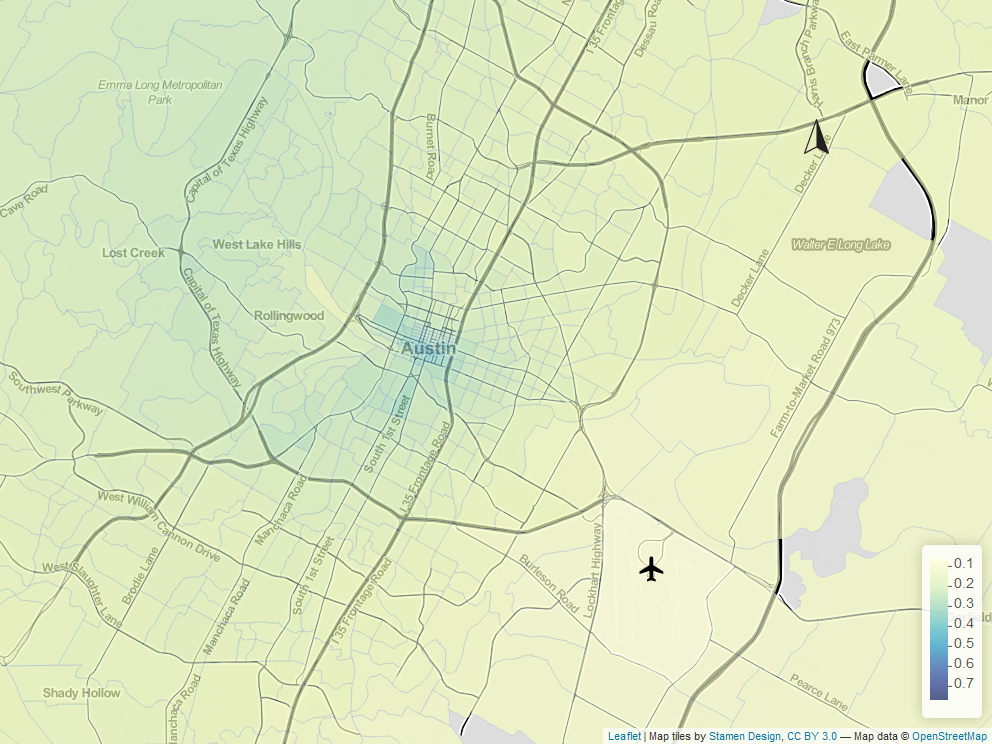
\includegraphics[width=\linewidth]{img/tailprob_34_74__142.png}
        \subcaption{Friday 9pm (weekday social mild traffic)}
        \label{fig:wages:appendix3:c}
    \end{minipage}
    \begin{minipage}[t]{0.48\linewidth}
        \centering
        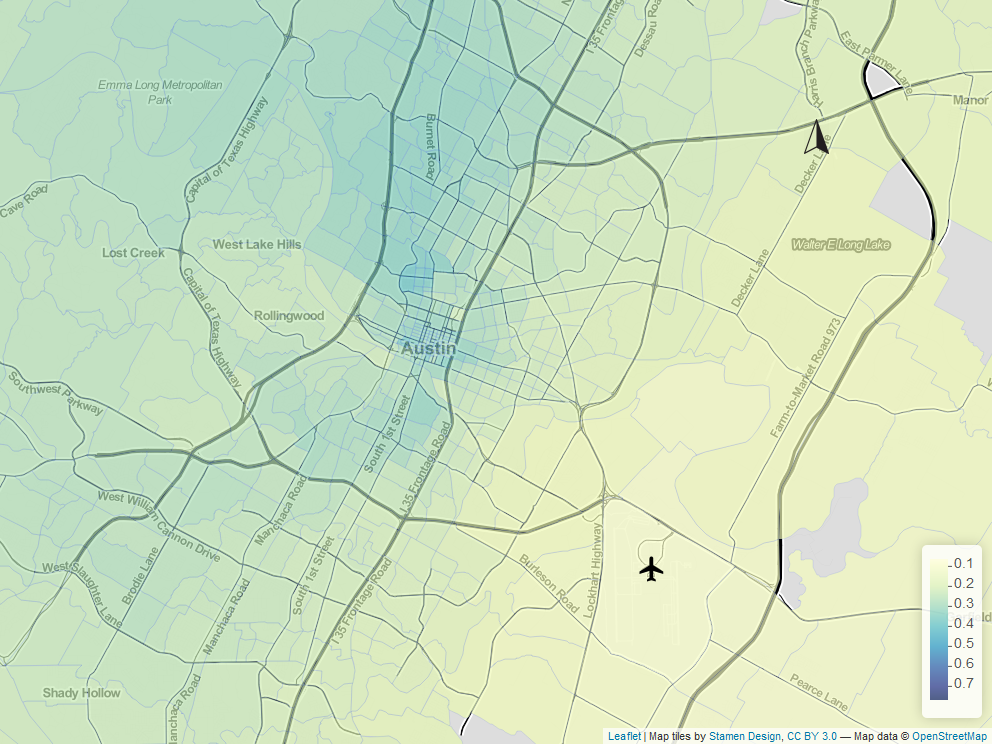
\includegraphics[width=\linewidth]{img/tailprob_34_74__168.png}
        \subcaption{Saturday 11pm (weekend social low traffic)}
        \label{fig:wages:appendix3:d}
    \end{minipage}
    \caption{Probability of exceeding \$34.74 in the next hour given a current location (living wage with costs for one adult with two children).}
    \label{fig:wages:appendix3}
\end{figure}

\section{Quantiles}
\label{appendix:quantiles}


\begin{figure}[htb]
    \centering
    \begin{minipage}[t]{0.48\linewidth}
        \centering
        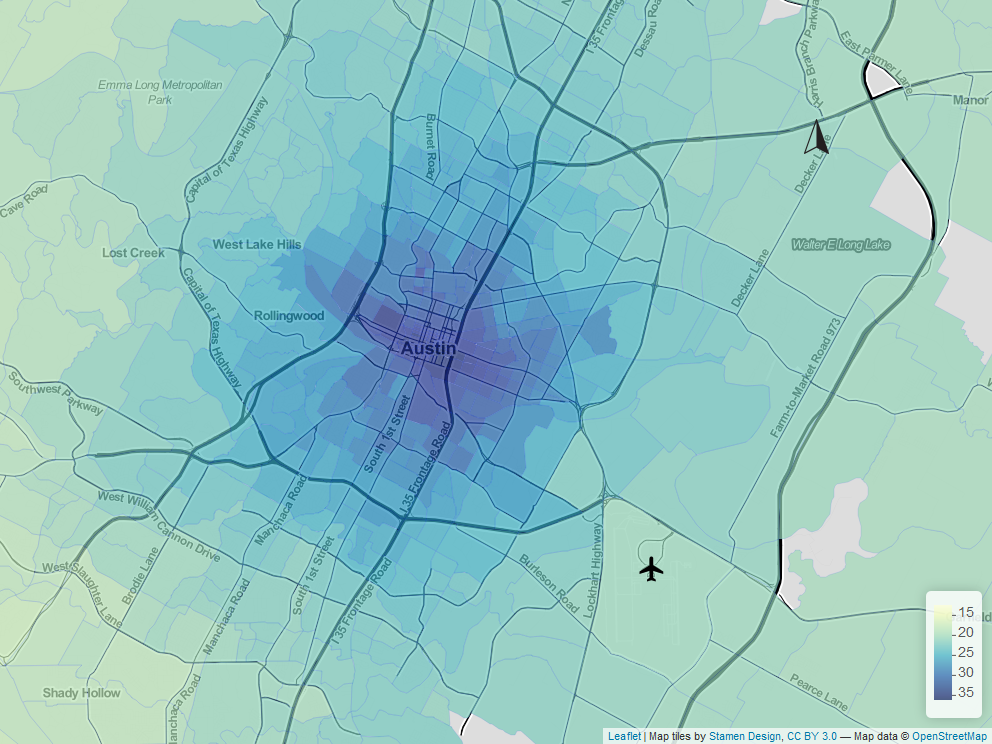
\includegraphics[width=\linewidth]{img/quantile_9_25.png}
        \subcaption{Sunday 8am (weekend low traffic)}
        \label{fig:quantiles:0.25:a}
    \end{minipage}
    \begin{minipage}[t]{0.48\linewidth}
        \centering
        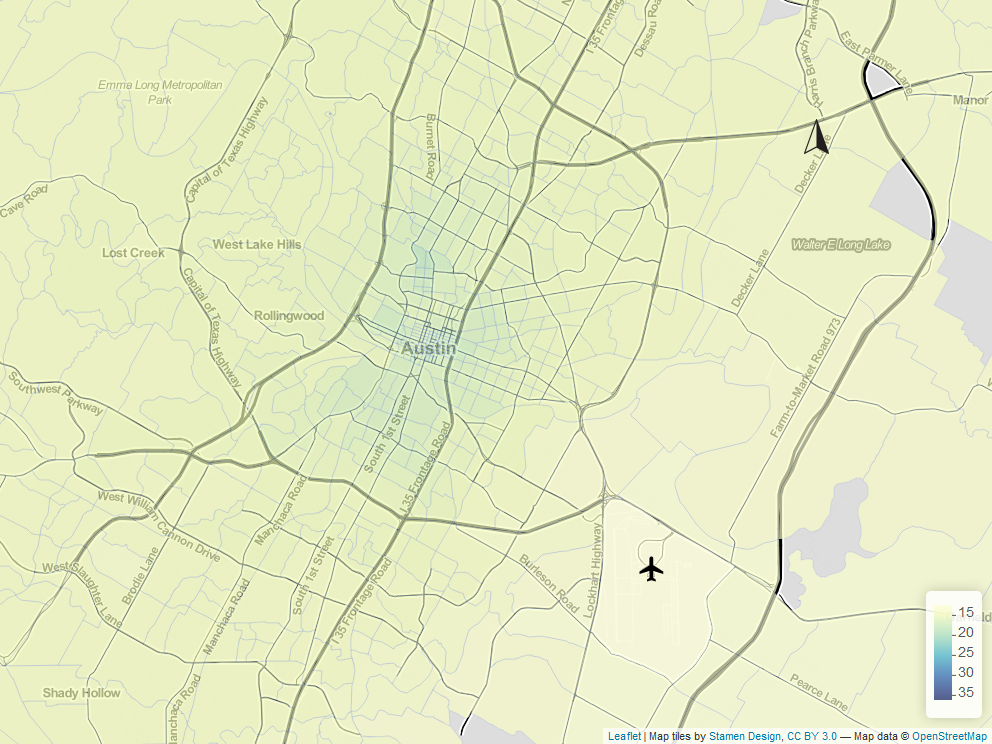
\includegraphics[width=\linewidth]{img/quantile_43_25.png}
        \subcaption{Monday 6pm (weekday rush hour)}
        \label{fig:quantiles:0.25:b}
    \end{minipage}\hfill
    \begin{minipage}[t]{.48\linewidth}
        \centering
        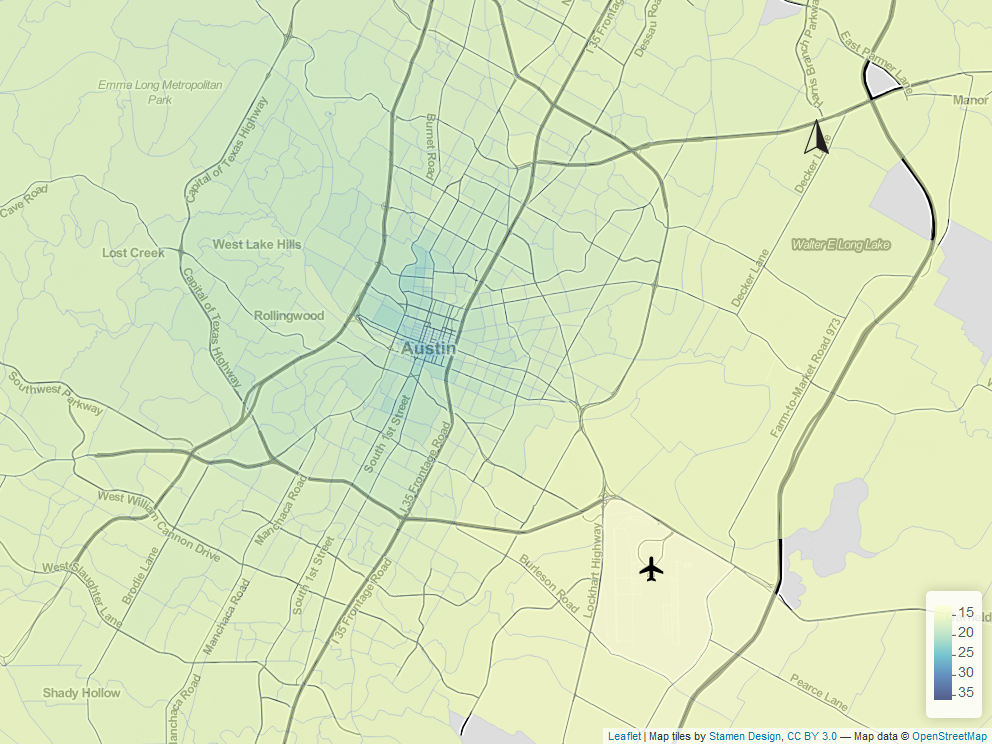
\includegraphics[width=\linewidth]{img/quantile_142_25.png}
        \subcaption{Friday 9pm (weekday social mild traffic)}
        \label{fig:quantiles:0.25:c}
    \end{minipage}
    \begin{minipage}[t]{0.48\linewidth}
        \centering
        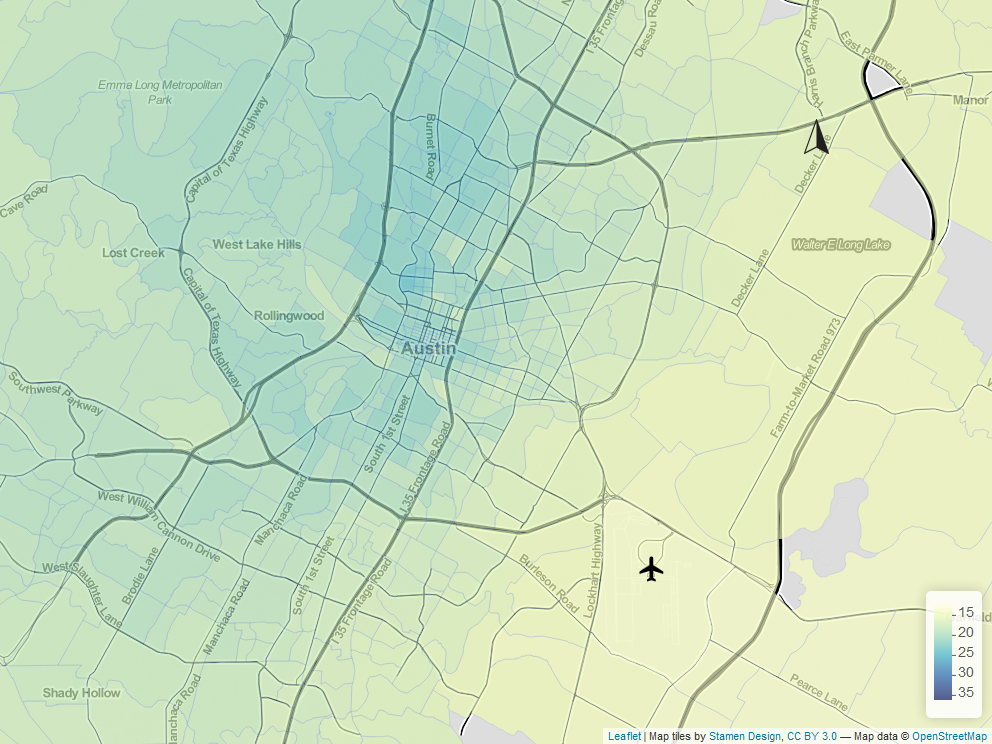
\includegraphics[width=\linewidth]{img/quantile_168_25.png}
        \subcaption{Saturday 11pm (weekend social low traffic)}
        \label{fig:quantiles:0.25:d}
    \end{minipage}
    \caption{Lower 25\% quantile of productivity for different times and locations.}
    \label{fig:quantiles:0.25}
\end{figure}



\begin{figure}[htb]
    \centering
    \begin{minipage}[t]{0.48\linewidth}
        \centering
        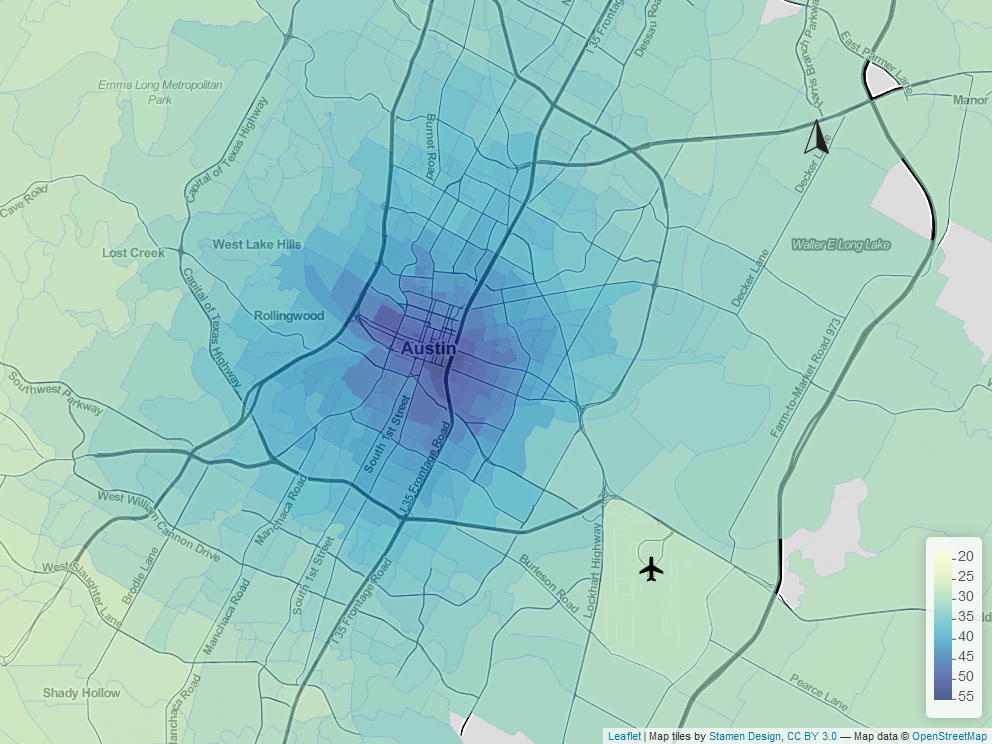
\includegraphics[width=\linewidth]{img/quantile_9_5.png}
        \subcaption{Sunday 8am (weekend low traffic)}
        \label{fig:quantiles:0.5:a}
    \end{minipage}
    \begin{minipage}[t]{0.48\linewidth}
        \centering
        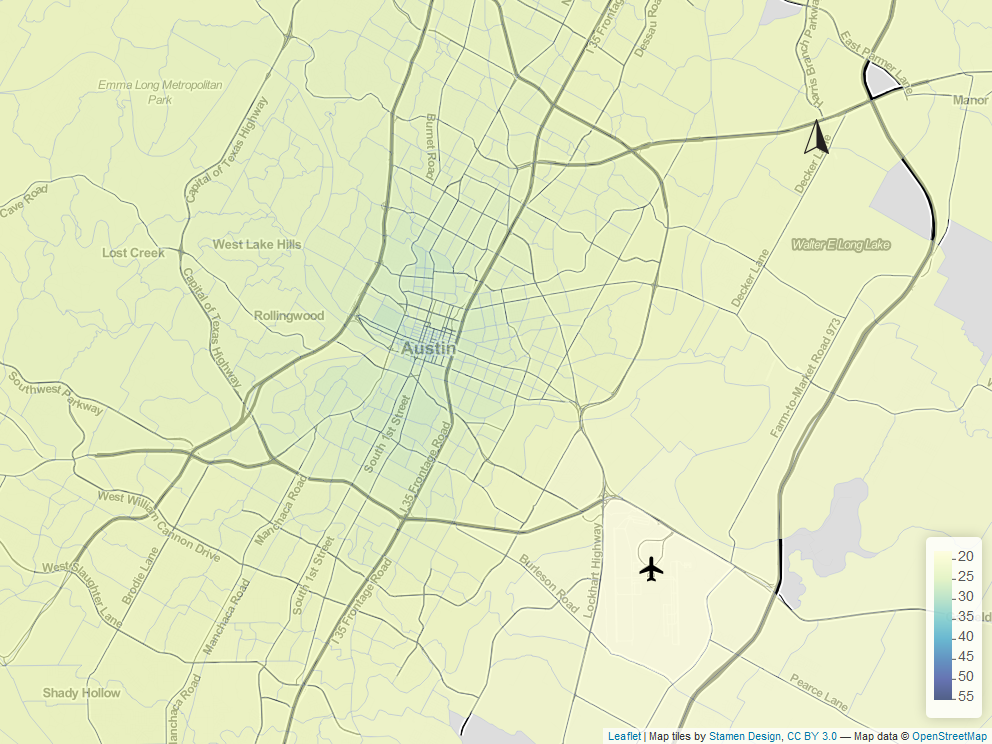
\includegraphics[width=\linewidth]{img/quantile_43_5.png}
        \subcaption{Monday 6pm (weekday rush hour)}
        \label{fig:quantiles:0.5:b}
    \end{minipage}\hfill
    \begin{minipage}[t]{.48\linewidth}
        \centering
        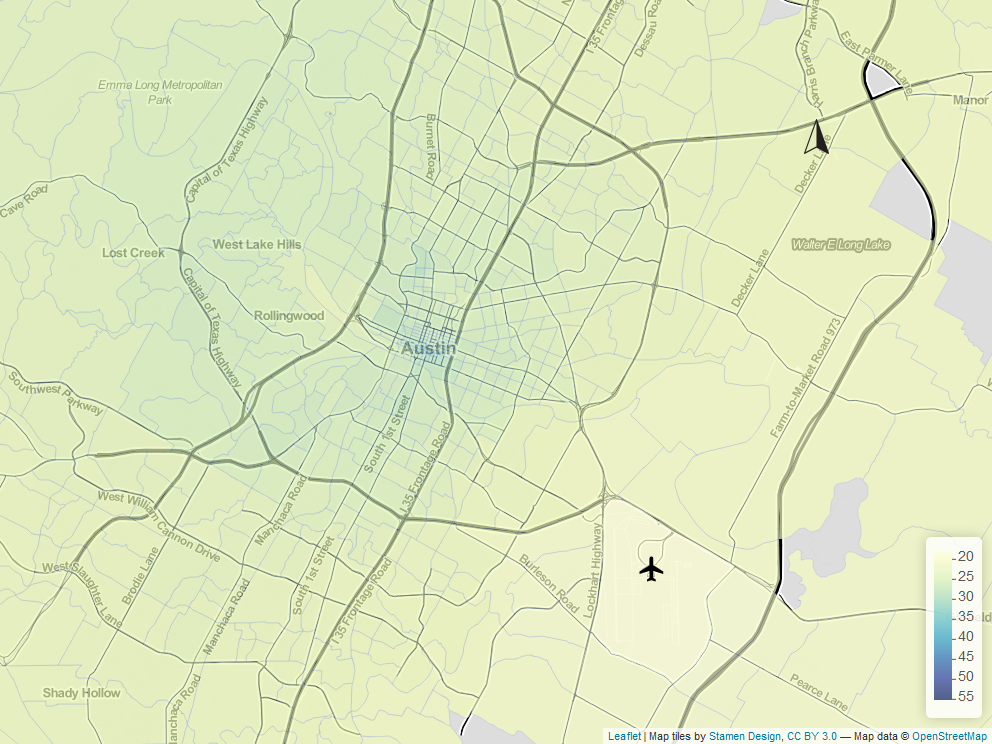
\includegraphics[width=\linewidth]{img/quantile_142_5.png}
        \subcaption{Friday 9pm (weekday social mild traffic)}
        \label{fig:quantiles:0.5:c}
    \end{minipage}
    \begin{minipage}[t]{0.48\linewidth}
        \centering
        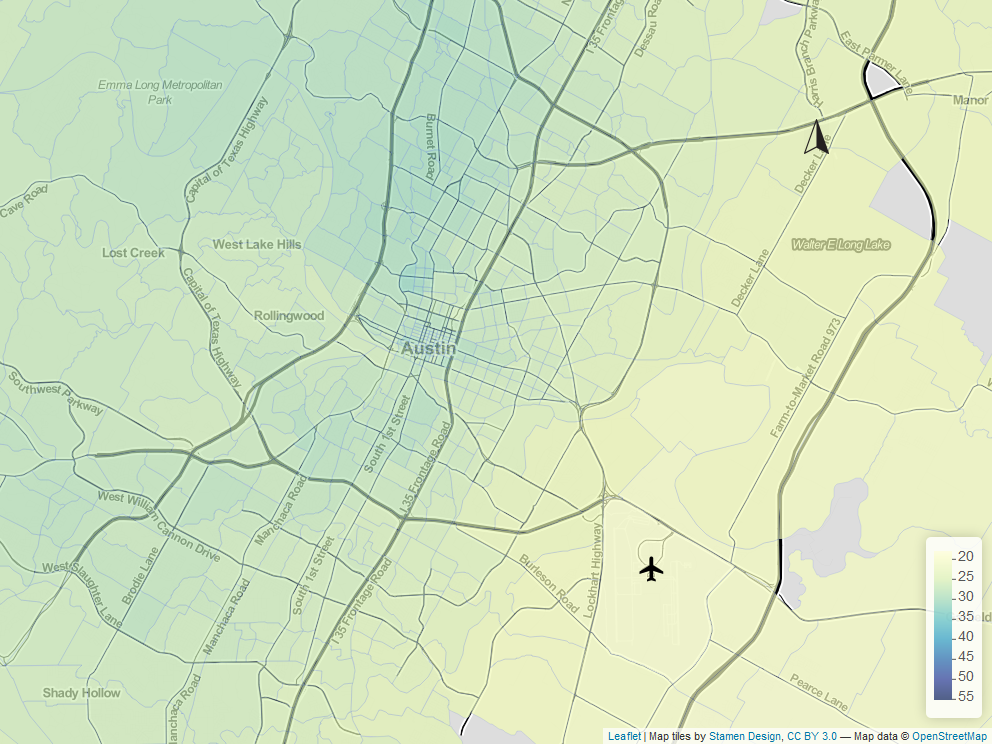
\includegraphics[width=\linewidth]{img/quantile_168_5.png}
        \subcaption{Saturday 11pm (weekend social low traffic)}
        \label{fig:quantiles:0.5:d}
    \end{minipage}
    \caption{Median of productivity for different times and locations.}
    \label{fig:quantiles:0.5}
\end{figure}

\bigskip
\begin{center}
{\large\bf SUPPLEMENTARY MATERIAL}
\end{center}

\begin{description}

\item[Title:] Brief description. (file type)

\item[R-package for  MYNEW routine:] R-package containing code to perform the diagnostic methods described in the article. The package also contains all datasets used as examples in the article. (GNU zipped tar file)

\item[HIV data set:] Data set used in the illustration of MYNEW method in Section~ 3.2. (.txt file)

\end{description}

\bibliographystyle{Chicago}

\bibliography{bibliography}

\end{document}
